\documentclass[11pt]{article}
\usepackage[margin=1in]{geometry}
\usepackage{natbib}
\usepackage{graphicx}
\usepackage{pdflscape}
\usepackage[T1]{fontenc}
\usepackage[utf8]{inputenc}
\usepackage{lmodern}
\usepackage{setspace}
\usepackage{parskip}
\usepackage{booktabs}
\usepackage[hidelinks]{hyperref}
\usepackage{float}
\usepackage{caption}
\usepackage{placeins}



\begin{document}

\section{Introduction}

The rapid expansion of environmental, social, and governance (ESG) reporting has made corporate environmental disclosure an important information channel for investors, regulators, and other stakeholders.
Environmental communication can enhance legitimacy and attract capital, but these benefits also create incentives for firms to present a favorable environmental image without achieving commensurate environmental performance \citep{delmas2011drivers}.
Greenwashing therefore arises when environmental communication creates a strategic divergence from the substantive environmental performance that could support that communication \citep{lyon2011greenwash,zhou2024environmental}.
This divergence reduces the credibility and decision usefulness of environmental information because stakeholders may interpret favorable narratives as evidence of environmental conduct that the firm's actual performance does not support \citep{christensen2021mandatory,zhou2024environmental}.
An important but unresolved question is whether the ordinary financial-statement audit can constrain this communication--performance divergence even when no separate sustainability assurance is provided.

Environmental narratives in annual reports generally fall outside the direct scope of the financial-statement audit opinion.
However, they are not necessarily isolated from the audit process.
ISA 720 and its Chinese counterpart, CAS 1521, require auditors to read other information and consider whether it is materially inconsistent with the audited financial statements or with knowledge obtained during the audit.
These requirements do not make the financial-statement auditor an assurer of environmental information.
They nevertheless create a limited institutional channel through which particular environmental statements may be compared with information obtained during the ordinary audit.
The possibility of such comparison depends on the content of the environmental statement.
General aspirations, policy slogans, and broad commitments usually provide few concrete points of comparison.
By contrast, statements describing environmental projects, technology adoption, capital investment, pollution remediation, equipment installation, regulatory rectification, or measurable environmental outcomes may contain factual anchors that have financial, operational, or compliance-related implications \citep{clarkson2004market,clarkson2008revisiting,barth1994estimation}.
Such statements may therefore intersect with information about assets, expenditures, cash flows, production processes, environmental obligations, penalties, or other matters encountered during the audit.
Accordingly, concrete action claims are more likely than symbolic claims to provide information that can be assessed with the auditor's existing knowledge of the client and its industry.

Audit firm industry specialization may make this evaluation more informative.
Industry-specialist auditors accumulate knowledge about clients' business models, production processes, technologies, regulatory environments, and typical financial relationships \citep{solomon1999industry,francis2011framework,reichelt2010national}.
This knowledge can help them recognize when several individually ambiguous signals form an unusual pattern, assess the risk associated with that pattern, and select more targeted follow-up procedures \citep{owhoso2002error,low2004effects,hammersley2006pattern}.
Applied to environmental narratives, industry expertise may improve the probability that an auditor recognizes a concrete environmental claim that is difficult to reconcile with the client's operations, financial information, or information obtained during the audit.
If a potential material inconsistency becomes salient, CAS 1521 provides a basis for discussing the matter with management, considering whether further work is necessary, and communicating an uncorrected material misstatement to those charged with governance.
This process may discourage environmental action claims that management cannot adequately support or reconcile with the firm's audited financial, operational, and compliance-related information.
To the extent that such unsupported claims inflate the substantive appearance of environmental disclosure relative to the firm's underlying environmental performance, their reduction narrows the gap captured by our measure of greenwashing.
This reasoning leads to our research question: Is audit firm industry specialization associated with less corporate greenwashing?

We examine this question using 15,381 firm-year observations for Chinese A-share listed firms from 2021 through 2024. 
We view greenwashing as the use of environmental language to create a favorable environmental image without corresponding substantive environmental improvement. 
Accordingly, we measure greenwashing as the within-industry-year divergence between a disclosure-side measure and an external environmental-performance score. 
Following the DeepGreen procedure \citep{xu2026deepgreen}, 
we use LLM-enabled semantic classification of annual-report text to distinguish substantive statements describing firm-specific environmental actions from symbolic statements such as aspirations, slogans, and general commitments. 
The resulting green implementation ratio (GI) is the share of classified environmental statements that are substantive. 
A GI approaching one indicates that the firm's identified environmental communication is predominantly supported by descriptions of concrete actions or improvements; 
a GI approaching zero indicates that it is predominantly symbolic. 
GI therefore captures the substantive effectiveness of the disclosure side, rather than the sheer amount of green language. 
Conventional measures based on environmental word counts, statement counts, report length, or textual tone primarily capture disclosure volume or rhetorical positivity; they combine substantive and symbolic communication and may increase when firms accumulate generic green language to project a favorable image \citep{lubloy2025quantifying,yu2020greenwashing,grewal2022unrepresentative,walker2012harm}. 
In contrast, the total number of classified statements captures disclosure quantity, while GI distinguishes the substantive component from that quantity by identifying whether the communication describes a concrete environmental action \citep{clarkson2008revisiting,hummel2016relationship,xu2026deepgreen}. 
We identify greenwashing when a relatively high GI is paired with comparatively weak external environmental performance; 
the resulting communication--performance gap is our greenwashing measure. 
We measure audit firm industry specialization using the audit firm's share of client operating revenue within an industry-year and a binary indicator of strong specialization equal to one when that share is at least 20 percent \citep{cai2007specialization,krishnan2003expertise}.
The analysis controls for financial, governance, and audit characteristics and includes year and industry fixed effects.
The main results show that audit firm industry specialization is negatively associated with corporate greenwashing. This negative association is robust across various specifications and robustness tests.

This study contributes to the literature in three ways.
First, it extends research on audit firm industry specialization and client disclosure quality by examining whether industry expertise is associated with the gap between environmental communication and environmental performance \citep{balsam2003auditor,dunn2004audit,reichelt2010national}.
Second, the study adds to greenwashing research by identifying a potential governance spillover from the ordinary financial-statement audit, rather than focusing only on firms' legitimacy incentives and external environmental scrutiny \citep{delmas2011drivers,lyon2011greenwash,marquis2016scrutiny}.
Third, the study uses semantic classification to distinguish substantive from symbolic environmental communication in a large-sample auditing setting \citep{baier2020textual,bilinski2024usefulness,xu2026deepgreen}.

The remainder of the paper develops the theoretical arguments, explains the measurement and research design, presents the empirical results, and concludes.

\section{Literature Review and Hypothesis Development}

\subsection{Greenwashing as an Action--Performance Divergence}

Environmental disclosure can reduce information asymmetry by helping investors and other stakeholders assess firms' environmental responsibilities, exposures, and performance \citep{healy2001information,verrecchia2001essays}.
Its usefulness depends on whether environmental communication provides a credible representation of underlying corporate conduct.
When firms use favorable environmental communication strategically, disclosure can obscure rather than clarify environmental performance.
Greenwashing is therefore commonly understood as a mismatch between positive environmental communication and the substantive environmental performance that could support that communication \citep{delmas2011drivers,lyon2011greenwash}.

Stakeholder expectations and legitimacy pressures increase the benefits of appearing environmentally responsible, whereas substantive environmental improvements may require costly changes in technology, production, and organizational practices \citep{delmas2011drivers}.
Firms may consequently rely on selective, exaggerated, or symbolic communication when outsiders cannot readily observe the underlying performance.
Prior research shows that institutional norms, external scrutiny, and the expected cost of having environmental claims challenged can affect firms' disclosure choices \citep{kim2015greenwash,marquis2016scrutiny,lyon2011greenwash}.
Taken together, these arguments suggest that greenwashing becomes more attractive when the benefits of a favorable environmental image exceed the expected costs of having unsupported, incomplete, or misleading claims challenged.

According to the measurement of greenwashing,
consistent with the greenwashing literature, our core concern is that firms may accumulate environmental-friendly language to construct a favorable image without achieving corresponding environmental improvement \citep{delmas2011drivers,lyon2011greenwash,marquis2016scrutiny}.
Conventional green-disclosure measures based on word counts, sentence counts, or overall disclosure volume capture the amount of environmental communication but may not distinguish concrete environmental implementation from symbolic or promotional language \citep{clarkson2008revisiting,hummel2016relationship,xu2026deepgreen}.
A firm may therefore disclose many environmental words or statements while providing little evidence of concrete action, whereas a smaller number of specific statements may be more informative when they describe actual implementation \citep{clarkson2008revisiting,marquis2016scrutiny}.
Conversely, a smaller number of specific statements may be more informative when those statements describe actual implementation. 
A useful disclosure-side measure must distinguish communication that describes firm-specific environmental action from communication that consists mainly of symbolic expression, 
and it must then be interpreted jointly with an independent measure of environmental performance.

We use the green implementation ratio (GI)\citep{xu2026deepgreen}, defined as the share of classified environmental communication that describes a substantive action rather than a symbolic statement. 
This choice builds on the distinction between hard and soft environmental disclosure: 
hard information contains more specific, verifiable, and decision-relevant content, 
whereas soft information more often consists of policies, principles, aspirations, or favorable descriptions \citep{clarkson2008revisiting,hummel2016relationship}. 
When GI approaches one, most identified environmental disclosure is supported, at least in its content, by descriptions of concrete actions or substantive improvements. 
When GI approaches zero, the disclosure is dominated by symbolic language or the firm has no classified environmental disclosure. 
Thus, a higher GI indicates stronger substantive effectiveness on the disclosure side, whereas a lower GI indicates a greater possibility of a communication--action disconnect. 

GI is consequently more closely aligned with the action side of the action--performance construct than raw disclosure counts, word frequency, sentiment, or overall environmental disclosure volume. A recent systematic review identifies measures based on disclosure quantity, report length, sustainability-word frequency, and sentiment as common ways to proxy for firms' symbolic environmental communication \citep{lubloy2025quantifying}. For example, the widely used decoupling measure of \citet{yu2020greenwashing} contrasts an ESG disclosure score---which reflects the amount of disclosed ESG data---with an ESG-performance score. Content-analysis studies similarly use report length, the frequency or proportion of sustainability terms, and sentiment to capture the extent, specificity, or tone of corporate communication \citep{grewal2022unrepresentative,walker2012harm,baier2020textual,bilinski2024usefulness}. 
These measures are valuable for capturing reporting intensity or rhetorical positivity, but quantity- and tone-based measures do not, on their own, distinguish firm-specific implementation from symbolic expression. A report may discuss a sustainability topic extensively, or use many favourable environmental terms, while masking other material environmental issues or providing no evidence that the firm implemented a project, adopted a technology, remediated pollution, or achieved a specified environmental outcome \citep{lubloy2025quantifying,clarkson2008revisiting,hummel2016relationship,xu2026deepgreen}. By semantically classifying environmental statements as substantive or symbolic, GI retains the scale of classified communication in its denominator while identifying the action-oriented component in its numerator. It therefore separates disclosure quantity from the substantive content of disclosure, which is the particular communication dimension relevant to our action--performance measure.

We identify greenwashing as the within-industry-year divergence between GI and an external environmental-performance score: greenwashing only when a relatively high GI is not matched by comparatively strong environmental performance \citep{delmas2011drivers,lyon2011greenwash,lubloy2025quantifying,xu2026deepgreen}.

\subsection{Environmental Action Claims as Points of Comparison}

The hard--soft disclosure distinction gives the measurement argument a direct auditing implication. 
Hard environmental information refers to relatively specific and verifiable content, such as environmental investments, performance indicators, expenditures, incidents, or progress toward specified targets. 
Soft information consists more often of general policies, principles, commitments, and favorable descriptions \citep{clarkson2008revisiting,hummel2016relationship}. 
The distinction matters here not simply because hard information is substantively richer, but because its specificity creates identifiable objects that an auditor may compare with financial statements and with knowledge obtained during the audit.

For example, a claim that an environmental equipment project has been implemented may have implications for capital expenditures, construction in progress, procurement, or payments. 
A pollution-remediation claim may relate to expenditures, environmental liabilities, provisions, or contingencies \citep{barth1994estimation,barth1997factors,li1997corporate}, 
while an environmental technology upgrade may be connected to equipment changes, production processes, operating costs, or industry-specific technical conditions \citep{clarkson2004market}. 
Symbolic statements generally lack these identifiable implications. 
Thus, GI links the measurement to the audit mechanism because it identifies the portion of environmental communication that is more likely to generate a concrete comparison point with information available to the auditor. 

CAS 1521 establishes the relevant procedural boundary.
When reading other information, the auditor considers whether it is materially inconsistent with the financial statements or with knowledge obtained during the audit and remains alert to indications that the other information may be materially misstated.
If an apparent material inconsistency arises, the auditor discusses the matter with management and considers whether additional procedures or communication are necessary.
Accordingly, CAS 1521 does not require auditors to verify all environmental claims or to provide sustainability assurance.
It does, however, provide a limited channel through which a concrete environmental claim may become relevant to the auditor when that claim intersects with available financial, operational, or compliance-related information.

\subsection{Industry Specialization and Recognition of Inconsistencies}

Industry specialization strengthens the information base relevant to this potential comparison.
Through repeated engagements, specialist audit firms develop knowledge about industry business models, production processes, regulatory requirements, technologies, cost structures, and reporting risks \citep{francis2011framework,reichelt2010national}.
This knowledge helps auditors form more precise expectations about the relationships among a client's operations, financial information, and industry conditions.
Experimental evidence indicates that industry specialists possess richer industry knowledge and are better able to identify errors or unusual patterns in industry-related information \citep{solomon1999industry,owhoso2002error}.
Industry specialization also affects audit risk assessments and planning decisions, including judgments about the nature and quality of subsequent audit procedures \citep{low2004effects}.
Hammersley (2006) further shows that industry specialists can identify complex error patterns formed by several individually ambiguous cues and can propose more discriminating follow-up procedures \citep{hammersley2006pattern}.

These studies support a inference about comparative recognition ability.
When an environmental action claim, a financial reporting item, and an operational or regulatory fact jointly form an unusual pattern, industry specialists may be better positioned to recognize that the pattern warrants attention.
For example, an assertion that a major environmental upgrade has been completed may be more informative to an industry specialist who understands the technology, production scale, expected investment, and operational consequences associated with that upgrade.
Similarly, a claim of comprehensive environmental rectification may be easier to evaluate when the auditor understands the client's exposure to industry regulation and the operational implications of the alleged rectification.
The relevant mechanism is that concrete claims increase the opportunity for comparison, while industry specialization improves the auditor's ability to interpret whether the available information forms a potentially inconsistent pattern.

\subsection{From Recognition to Informed Questioning}

Recognition of a potential inconsistency may affect the information environment surrounding management's disclosure choices.
Under CAS 1521, an auditor who identifies an apparent material inconsistency discusses the matter with management, considers the explanations and supporting information provided, and determines whether further action or communication is necessary.
Industry knowledge can make these questions more specific because the auditor can relate management's explanation to the client's production activities, financial reporting, technology, and regulatory setting.
More informed questioning implies that management may face greater difficulty sustaining a concrete claim that is difficult to reconcile with information already available to the auditor.

This reasoning is consistent with evidence that auditing can influence disclosure choices beyond the audited financial statements and that auditor industry specialization is associated with client disclosure quality \citep{schroeder2016impact,dunn2004audit}.
A firm may still disclose environmental actions for legitimacy or capital-market reasons, but an industry specialist may increase the expected cost of presenting unsupported action claims as evidence of strong environmental performance.
The resulting prediction is an association between specialization and less greenwashing.

\subsection{Scope Conditions and Hypothesis}

Several considerations limit this predicted association.
The auditor's responsibility for other information is narrower than the responsibility arising in a separate sustainability assurance engagement.
Financial-statement audit expertise may also be insufficient to evaluate the scientific or technical substance of some environmental claims.
Some environmental actions may be implemented through arrangements that have no clear or material accounting manifestation.
Firms also retain strong legitimacy and capital-market incentives to maintain favorable environmental narratives \citep{delmas2011drivers,healy2001information,verrecchia2001essays}.
Dedicated sustainability assurance remains a distinct governance mechanism with different procedures, expertise, and responsibilities \citep{simnett2009assurance,pflugrath2011impact,cohen2015csr}.
These limitations imply that industry specialization should not be expected to eliminate greenwashing or to affect every environmental statement.
They do not, however, rule out a detectable average association when firms' concrete environmental claims provide points of comparison and specialist auditors possess a comparative advantage in recognizing inconsistent patterns.
We therefore state the following hypothesis:

\medskip
\noindent\textbf{H1: Audit firm industry specialization is negatively associated with corporate greenwashing.}
\medskip

\section{Research Design}

\subsection{Sample Selection and Data Sources}

Our initial sample consists of Chinese A-share listed firms from 2021 through 2024. 
We exclude firms designated as *ST, ST, or PT during the sample period, as these firms may exhibit abnormal financial conditions and operating characteristics.
Annual reports are obtained from the CNINFO website, and financial, corporate-governance, audit, 
and full-market audit-client data are primarily obtained from the China Stock Market \& Accounting Research (CSMAR) database. 
We use Huazheng environmental scores as the external measure of firms' environmental performance. 
The annual-report text and environmental scores are used to construct the greenwashing measure, 
while the full-market audit-client data are used to calculate audit firm industry specialization. 
Financial, governance, and audit data provide the control variables. 
Following the industry-classification convention commonly applied to Chinese listed firms \citep{gul2010ownership}, 
we classify manufacturing firms at the CSRC two-digit industry level and firms in other sectors at the CSRC one-digit industry level.

Our sample-selection procedure is designed to ensure the completeness of the annual-report text, the feasibility of the green-disclosure classification, and the availability of data required for the empirical analysis. 
We first retain firm-years for which the relevant annual-report text can be extracted completely and the green-disclosure identification procedure can be completed. 
Firm-years with extraction or classification failures are treated as incomplete rather than as having zero green disclosure. 
We combine the valid textual classifications with Huazheng environmental scores to form the dependent-variable panel. 
We then match this panel to audit firm industry-specialization measures calculated from the full A-share audit market. 
Finally, we exclude observations with substantial missing financial, governance, or audit data and require nonmissing values for the dependent variable, 
both main specialization measures, all control variables, firm and year identifiers, and the industry code used in the analysis. 
Table~\ref{tab:sample_selection} summarizes the sample-selection procedure. 
Following common practice, we winsorize continuous control variables at the 1st and 99th percentiles to limit the influence of extreme accounting ratios and growth rates. 
We do not winsorize the specialization measures because their upper-tail values represent economically meaningful audit-market concentration rather than mechanical outliers. 
We also retain the original Greenwashing measure because its tail observations capture firms with unusually large communication--performance gaps, which constitute the substantive phenomenon examined in this study.
\begin{table}[htbp]
    \centering
    \caption{Sample Selection}
    \label{tab:sample_selection}
    \begin{tabular}{p{0.78\textwidth}r}
        \toprule
        Sample-selection procedure & Firm-years \\
        \midrule
        Initial A-share firm-year panel, 2021--2024 & 18,077 \\
        Less: incomplete annual-report text extraction or unsuccessful green-disclosure classification, or insufficient industry-year variation to construct the continuous greenwashing measure & (1,594) \\
        Less: missing financial control variables & (700) \\
        Less: missing corporate-governance control variables & (381) \\
        Less: missing audit control variables & (21) \\
        \midrule
        Final regression sample & 15,381 \\
        \bottomrule
    \end{tabular}

    \par\smallskip
    \begin{minipage}{0.95\textwidth}
        \footnotesize
        \textit{Notes:} The initial panel excludes firms designated as \texttt{*ST}, \texttt{ST}, or \texttt{PT} during the sample period. Firm-years with incomplete text extraction or unsuccessful green-disclosure classification are treated as incomplete observations rather than as zero environmental disclosure. The final sample contains 4,604 unique firms over 2021--2024.
    \end{minipage}
    \end{table}

\subsection{Variable Measurement}

\subsubsection{Measure of Greenwashing}

We construct the dependent variable by adapting the DeepGreen procedure \citep{xu2026deepgreen}. 
We first extract the ``Environmental Information'' section from each annual report\footnote{We segment the Chinese text using Jieba, remove terms contained in the HIT Stopword List}. 
Layer A identifies environmentally relevant terms, after which we retrieve the complete sentence containing each identified term from the unsegmented report text. 
Layer B classifies each resulting keyword--sentence pair as substantive or symbolic environmental disclosure \footnote{The two LLM classification layers using Qwen 3.6, a Qwen3-family model \citep{yang2025qwen3}.}. 
The reliability of the semantic classifications is assessed through an independent human-validation exercise reported in Appendix~\ref{sec:semantic-validation}.

Substantive disclosure describes a concrete environmental action undertaken by the firm or its subsidiaries, such as implementing a project, adopting a technology, or taking a specific pollution-control measure. 
Symbolic disclosure includes general aspirations, slogans, policy restatements, and other statements that do not identify a concrete corporate action.
Conventional measures based on the total number of environmental words or statements capture disclosure quantity but cannot distinguish substantive environmental actions from symbolic language. 
We therefore identify environmental statements and classify them according to whether they describe a concrete firm-level action. 
Let the total number of classified environmental statements be the sum of substantive statements and symbolic statements. 
The total reflects the scale of environmental communication, 
while the substantive share---GI---identifies the effective portion of that communication. 
When GI approaches one, the disclosure is predominantly action-oriented; 
when GI approaches zero, it is predominantly symbolic or absent. 
This makes GI particularly suitable for capturing the disclosure-side effectiveness of an action--performance divergence, 
while the external Huazheng score supplies the separate performance dimension.

We aggregate the Layer B classifications at the firm-year level. 
Let \(S_{i,t}\) denote the number of keyword--sentence pairs classified as substantive and \(P_{i,t}\) the number classified as symbolic. 
The green implementation ratio is

\[
GI_{i,t}=\frac{S_{i,t}}{S_{i,t}+P_{i,t}}.
\]

The unit of analysis is the keyword--sentence pair rather than the unique sentence; 
consequently, a sentence containing multiple environmental keywords may contribute more than one classification. 
Observations for which the text-extraction or classification procedure does not yield any valid keyword--sentence pairs are treated as missing rather than as zero environmental disclosure. 


Our primary measure compares environmental communication with external environmental performance. 
Firms in different industries may have systematically different opportunities, technologies, regulatory exposure, 
and disclosure practices; standardizing across the pooled sample could therefore confound relative greenwashing with cross-industry differences. 
Following the recommendation that communication and performance components be benchmarked against industry peers rather than the pooled sample \citep{lubloy2025quantifying,yu2020greenwashing}, 
we standardize \(GI\) and the Huazheng environmental score within each industry-year group. 
The industry classification is the same as that used for audit firm industry specialization. 
This within-industry-year normalization follows the peer-relative logic of prior decoupling measures, 
while addressing the concern that disclosure practices and environmental performance differ systematically across industries \citep{yu2020greenwashing,lubloy2025quantifying}. 
For each component, the z-score is calculated using the corresponding industry-year mean and sample standard deviation (\(ddof=1\)). We define

\[
Greenwashing_{i,t}=GI\_z_{i,t}-ESGE\_z_{i,t}.
\]

This difference measure follows the broader decoupling approach that compares a communication-side indicator with an independently assessed performance indicator \citep{walker2012harm,yu2020greenwashing,lubloy2025quantifying}. 
A higher value indicates that a firm's substantive share of green communication is high relative to its industry-year peers while its externally assessed environmental performance is comparatively low, 
and therefore represents a larger communication--performance gap. 
As an alternative measure, we construct a binary indicator equal to one when \(GI\) is strictly above its industry-year mean and the Huazheng environmental score is strictly below its industry-year mean, and zero otherwise\citep{xu2026deepgreen}. 

\subsubsection{Measures of Audit Firm Industry Specialization}

Our explanatory variable measures specialization at the audit-firm level. Audit firms are identified by the stable CSMAR institution identifier. Following the market-share approach used in prior industry-expertise research \citep{cai2007specialization,krishnan2003expertise}, we calculate specialization from the full A-share audit market. 

Let \(Revenue_{i,t}\) be client operating revenue, \(a\) index audit firms, and \(j\) index industries. Our primary continuous measure, \(IMS\), is

\[
IMS_{a,j,t}=\frac{\sum_{i\in(a,j,t)}Revenue_{i,t}}
{\sum_{i\in(j,t)}Revenue_{i,t}}.
\]

The numerator is the operating revenue of all valid A-share clients audited by firm \(a\) in industry \(j\) and year \(t\), and the denominator is the operating revenue of all valid A-share firms in that industry-year. We include only observations with positive operating revenue and nonmissing audit-firm and industry identifiers. The resulting audit-firm--industry--year measure is matched to each client using year, audit-firm identifier, and this mixed industry code. An unmatched specialization observation remains missing.

We define \(IMS\_D\) as one when \(IMS\) is at least 20 percent and zero otherwise.

\subsubsection{Control Variables}

We include financial, governance, and audit controls that may be associated with firms' environmental disclosure and performance or with the selection of specialist auditors \citep{marquis2016scrutiny,reichelt2010national,defond2014review}. 
Financial controls comprise firm size (\(Size\)), measured as the natural logarithm of total assets; leverage (\(Lev\)), measured as total liabilities divided by total assets; 
return on assets (\(ROA\)), measured as net profit divided by total assets; operating cash flow (\(CFO\)), measured as operating net cash flow divided by total assets; 
sales growth (\(Growth\)), measured as current-year operating revenue divided by prior-year operating revenue minus one; 
and listing age (\(FirmAge\)), measured as the number of years since the firm's initial public listing. 
Growth is first calculated using consecutive-year revenue observations in the full-market financial data and is then matched to the research panel, 
which avoids creating artificial lags within the selected sample.

Governance controls comprise state ownership (\(SOE\)), an indicator equal to one when the CSMAR actual-controller type is state-owned and zero otherwise; 
CEO--chair duality (\(Dual\)); board size (\(BoardSize\)), measured as the natural logarithm of the number of directors; 
and the proportion of independent directors (\(Indep\)). 
Audit controls comprise an indicator for a Big Four auditor (\(Big4\)); audit fees (\(LnAuditFee\)), measured as the natural logarithm of total audit fees; 
auditor tenure (\(AuditorTenure\)); and an indicator for an audit-firm change (\(IsChangeFirm\)), coded as one if the firm appoints a different audit firm in the current year than in the preceding year, and zero otherwise. 
These audit controls help distinguish industry specialization from general audit-firm brand, audit effort, accumulated client knowledge, and changes in the auditor--client relationship \citep{defond2014review}. 
Values that do not satisfy the required positive-denominator or logarithm conditions, observations with nonconsecutive years for growth, and undefined or infinite ratios are treated as missing.

\subsection{Empirical Model}

We estimate the following pooled OLS model:
\[
Greenwashing_{i,t}=\alpha+\beta Specialization_{i,t}+\gamma'Controls_{i,t}+YearFE_t+IndustryFE_j+\varepsilon_{i,t}.
\]
The dependent variable is the continuous greenwashing measure. \(Specialization\) is alternatively \(IMS\) and \(IMS\_D\), and \(Controls\) contains the financial, governance, and audit variables defined above. The primary specification includes year and industry fixed effects, using the industry classification described above, and standard errors clustered by firm. H1 predicts \(\beta<0\). We estimate successive specifications containing only specialization, then adding financial controls, governance controls, audit controls, and finally year and industry fixed effects. We also estimate the complete model with industry-clustered standard errors. All specifications use the same 15,381 firm-year observations.

\section{Empirical Results}

\subsection{Descriptive Statistics}

Table~\ref{tab:descriptive-statistics} presents descriptive statistics for the common regression sample. 
Greenwashing has a mean close to zero by construction because both its components are standardized within industry-year groups. 
The measure captures the relative distance between environmental communication and environmental performance. 
Its standard deviation is 1.337, and the interquartile range extends from -0.820 to 0.898. 
This dispersion indicates considerable variation across firms in the degree to which their substantive environmental communication exceeds or falls short of their relative environmental performance.
The mean \(IMS\) is 0.070, while 5.7 percent of firm-years are audited by firms meeting the 20 percent strong-specialization threshold. 
This tail share indicates identifiable variation in strong industry expertise and provides a basis for comparing clients of strong specialists with other clients.
The average leverage ratio is 40.97 percent, suggesting that firms face debt-related financial pressure.
State-controlled firms account for 27.7 percent of the sample, highlighting the importance of regulatory and political expectations in shaping environmental disclosure. 
Big Four clients account for only 5.5 percent of firm-years, whereas auditor changes occur in 11.5 percent, suggesting that most firms are served by non-Big Four auditors and maintain relatively stable auditor–client relationships.

\subsection{Correlation Analysis}

Table~\ref{tab:correlations} reports the pairwise correlations. 
Greenwashing is negatively correlated with \(IMS\) (Pearson = -0.054) and \(IMS\_D\) (Spearman = -0.033), providing preliminary evidence consistent with H1: clients of auditors with greater industry expertise tend to exhibit a smaller gap between environmental communication and environmental performance. 
These unconditional associations are modest, as expected because firms' financial characteristics, governance, auditor choice, and industry conditions may jointly affect both specialization and greenwashing; the multivariate analysis therefore evaluates whether the association persists after accounting for these factors. 
The 0.402 correlation between \(IMS\) and \(IMS\_D\) reflects that \(IMS\_D\) is a threshold-based representation of \(IMS\). 
Among the controls, the largest correlation is 0.698 between Size and LnAuditFee, consistent with larger firms requiring greater audit effort and paying higher audit fees.

\subsection{Baseline Regression Results}

We estimate a sequence of nested regression models to examine the association between audit firm industry specialization and corporate greenwashing. 
Model (1) includes only the specialization measure, \(IMS\) or \(IMS_D\), and provides the unconditional association between auditor industry specialization and greenwashing. 
Model (2) adds financial controls, including firm size, leverage, profitability, operating cash flow, sales growth, and firm age, to account for differences in firms’ financial condition, operating performance, and life cycle. 
Model (3) further incorporates corporate-governance controls, including state ownership, CEO–chair duality, board size, and the proportion of independent directors, because governance structures may affect both auditor selection and the credibility of environmental disclosure. 
Model (4) adds audit-related controls, including Big Four affiliation, audit fees, auditor tenure, and auditor changes, allowing the analysis to distinguish industry specialization from auditor reputation, audit effort, accumulated client knowledge, and changes in the auditor–client relationship.
All four model specifications include year and industry fixed effects.

Tables~\ref{tab:baseline-regressions-ims} and \ref{tab:baseline-regressions-imsd} report the baseline regression results. 
Across all specifications, the coefficients on both \(IMS\) and \(IMS_D\) are negative, consistent with H1. 
In the most comprehensive specification, column (4), the coefficient on \(IMS\) is \(-0.4829\) and statistically significant at the 5 percent level. 
Given the definition of \(IMS\), this estimate implies that a 0.10 increase in an audit firm’s industry market share is associated with an approximately 0.0483 reduction in the Greenwashing measure, 
conditional on the control variables and year and industry fixed effects. 
The coefficient on \(IMS_D\) in column (4) is \(-0.1434\) and significant at the 10 percent level. 
Thus, relative to firms audited by non--specialized auditors, firms audited by auditors whose industry market share reaches the 20 percent specialization threshold exhibit, on average, a Greenwashing measure that is approximately 0.143 lower, conditional on the included controls and fixed effects. 
The negative and statistically significant coefficients across the two alternative specialization measures provide support for H1. As an additional check, Appendix~\ref{sec:baseline-robustness} examines whether the baseline inference is sensitive to alternative standard-error clustering schemes.

\clearpage
\begin{landscape}
    \vspace*{-1.5cm}

    \begin{center}
    
    \captionof{table}{Descriptive Statistics}
    \label{tab:descriptive-statistics}
    
    \scriptsize
    \resizebox{0.7\linewidth}{!}{%
    \begin{tabular}{lrrrrrrrr}\hline
    Variable & N & Mean & Std. Dev. & Min & 25th Pctl. & Median & 75th Pctl. & Max\\\hline
    Greenwashing&15,381&-0.0021&1.3366&-7.4995&-0.8204&-0.0291&0.8979&5.0962\\
IMS&15,381&0.0698&0.0817&0.0000&0.0152&0.0420&0.0983&0.7307\\
IMS\_D&15,381&0.0573&0.2324&0.0000&0.0000&0.0000&0.0000&1.0000\\
Size&15,381&22.3249&1.2148&20.1877&21.4376&22.1117&23.0181&26.0914\\
Lev&15,381&0.4097&0.2015&0.0557&0.2490&0.4012&0.5534&0.8994\\
ROA&15,381&0.0269&0.0644&-0.2226&0.0064&0.0310&0.0608&0.1909\\
CFO&15,381&0.0477&0.0644&-0.1363&0.0110&0.0459&0.0847&0.2311\\
Growth&15,381&0.0957&0.3074&-0.5521&-0.0708&0.0605&0.2086&1.5243\\
FirmAge&15,381&11.2589&8.7381&0.0000&4.0000&9.0000&17.0000&30.2000\\
SOE&15,381&0.2768&0.4474&0.0000&0.0000&0.0000&1.0000&1.0000\\
Dual&15,381&0.3439&0.4750&0.0000&0.0000&0.0000&1.0000&1.0000\\
BoardSize&15,381&2.1129&0.2198&1.6094&1.9459&2.1972&2.1972&2.7081\\
Indep&15,381&0.3826&0.0589&0.2727&0.3333&0.3750&0.4286&0.5714\\
Big4&15,381&0.0555&0.2289&0.0000&0.0000&0.0000&0.0000&1.0000\\
AuditFee&15,381&14.0021&0.5682&12.8992&13.5924&13.9108&14.3163&15.8304\\
Tenure&15,381&7.9131&6.0436&1.0000&3.0000&6.0000&11.0000&27.0000\\
AuditorChange&15,381&0.1151&0.3191&0.0000&0.0000&0.0000&0.0000&1.0000\\
    \\\hline
    \end{tabular}}
    
    \vspace{3pt}
    
    \begin{minipage}{0.75\linewidth}
    \footnotesize
    \textit{Notes:} This table reports descriptive statistics for all variables. All statistics are based on 15,381 firm-year observations.
    \end{minipage}
    
    \vspace{8pt}
    
    \captionof{table}{Pairwise Correlations}
    \label{tab:correlations}
    
    \resizebox{1\linewidth}{!}{%
    \begin{tabular}{lrrrrrrrrrrrrrrrrr}\hline
    Variables &
    (1) &
    (2) &
    (3) &
    (4) &
    (5) &
    (6) &
    (7) &
    (8) &
    (9) &
    (10) &
    (11) &
    (12) &
    (13) &
    (14) &
    (15) &
    (16) &
    (17)\\\hline
    
    (1) Greenwashing & 1.000 &  &  &  &  &  &  &  &  &  &  &  &  &  &  &  & \\
(2) IMS & \textbf{-0.054} & 1.000 &  &  &  &  &  &  &  &  &  &  &  &  &  &  & \\
(3) IMS\_D & \textbf{-0.033} & \textbf{0.402} & 1.000 &  &  &  &  &  &  &  &  &  &  &  &  &  & \\
(4) Size & \textbf{-0.113} & \textbf{0.163} & \textbf{0.105} & 1.000 &  &  &  &  &  &  &  &  &  &  &  &  & \\
(5) Lev & -0.013 & -0.003 & \textbf{0.024} & \textbf{0.430} & 1.000 &  &  &  &  &  &  &  &  &  &  &  & \\
(6) ROA & \textbf{-0.017} & \textbf{0.099} & \textbf{0.036} & \textbf{0.106} & \textbf{-0.347} & 1.000 &  &  &  &  &  &  &  &  &  &  & \\
(7) CFO & \textbf{-0.023} & \textbf{0.101} & \textbf{0.064} & \textbf{0.124} & \textbf{-0.153} & \textbf{0.489} & 1.000 &  &  &  &  &  &  &  &  &  & \\
(8) Growth & 0.000 & 0.001 & -0.013 & \textbf{0.033} & \textbf{0.034} & \textbf{0.300} & \textbf{0.082} & 1.000 &  &  &  &  &  &  &  &  & \\
(9) FirmAge & \textbf{-0.025} & \textbf{-0.021} & \textbf{0.039} & \textbf{0.429} & \textbf{0.310} & \textbf{-0.125} & \textbf{-0.018} & \textbf{-0.074} & 1.000 &  &  &  &  &  &  &  & \\
(10) SOE & \textbf{-0.034} & \textbf{-0.029} & \textbf{0.029} & \textbf{0.337} & \textbf{0.231} & \textbf{-0.072} & -0.014 & \textbf{-0.044} & \textbf{0.443} & 1.000 &  &  &  &  &  &  & \\
(11) Dual & 0.001 & \textbf{0.022} & \textbf{-0.031} & \textbf{-0.190} & \textbf{-0.118} & 0.011 & -0.007 & \textbf{0.027} & \textbf{-0.250} & \textbf{-0.310} & 1.000 &  &  &  &  &  & \\
(12) BoardSize & \textbf{-0.019} & \textbf{0.036} & \textbf{0.036} & \textbf{0.276} & \textbf{0.131} & \textbf{0.035} & \textbf{0.050} & 0.009 & \textbf{0.218} & \textbf{0.306} & \textbf{-0.198} & 1.000 &  &  &  &  & \\
(13) Indep & -0.010 & 0.004 & -0.004 & \textbf{-0.074} & \textbf{-0.046} & -0.001 & 0.002 & -0.001 & \textbf{-0.067} & \textbf{-0.140} & \textbf{0.139} & \textbf{-0.430} & 1.000 &  &  &  & \\
(14) Big4 & \textbf{-0.080} & \textbf{0.118} & \textbf{0.120} & \textbf{0.211} & \textbf{0.059} & \textbf{0.044} & \textbf{0.085} & 0.009 & \textbf{0.040} & \textbf{0.070} & \textbf{-0.037} & \textbf{0.074} & -0.013 & 1.000 &  &  & \\
(15) AuditFee & \textbf{-0.100} & \textbf{0.168} & \textbf{0.112} & \textbf{0.698} & \textbf{0.382} & \textbf{-0.055} & \textbf{0.087} & \textbf{-0.025} & \textbf{0.313} & \textbf{0.164} & \textbf{-0.098} & \textbf{0.178} & \textbf{-0.033} & \textbf{0.299} & 1.000 &  & \\
(16) Tenure & \textbf{0.034} & \textbf{0.081} & \textbf{0.051} & \textbf{0.069} & 0.011 & \textbf{0.062} & \textbf{0.061} & -0.006 & \textbf{0.135} & \textbf{-0.184} & \textbf{0.041} & \textbf{0.028} & \textbf{-0.027} & \textbf{-0.060} & \textbf{0.068} & 1.000 & \\
(17) AuditorChange & -0.011 & \textbf{-0.068} & 0.007 & \textbf{0.059} & \textbf{0.053} & \textbf{-0.071} & \textbf{-0.034} & \textbf{-0.044} & \textbf{0.122} & \textbf{0.170} & \textbf{-0.057} & \textbf{0.052} & \textbf{-0.029} & \textbf{0.022} & \textbf{0.030} & \textbf{-0.554} & 1.000\\
    \\\hline
    \end{tabular}}
    
    \vspace{3pt}
    
    \begin{minipage}{0.98\linewidth}
    \footnotesize
    \textit{Notes:} This table reports Pearson correlations when both variables are continuous and Spearman correlations when either variable is binary. Coefficients in bold are significant at the 5 percent level using two-tailed tests. Variables are numbered as follows: (1) Greenwashing, (2) IMS, (3) IMS\_D, (4) Size, (5) Lev, (6) ROA, (7) CFO, (8) Growth, (9) FirmAge, (10) SOE, (11) Dual, (12) BoardSize, (13) IndDirector, (14) Big4, (15) AuditFee, (16) Tenure, and (17) AuditorChange. All statistics are based on 15,381 firm-year observations.
    \end{minipage}
    
    \end{center}
    
    \end{landscape}
    
\clearpage
\begin{table}[htbp]
\centering\caption{Audit Firm Industry Specialization and Corporate Greenwashing: IMS}\label{tab:baseline-regressions-ims}
\footnotesize
\setlength{\tabcolsep}{6pt}
\renewcommand{\arraystretch}{1.12}
\resizebox{0.87\textwidth}{!}{%
\begin{tabular}{@{}lcccc@{}}\hline
&(1)&(2)&(3)&(4)\\[1pt]\hline
IMS & \shortstack{-1.0488***\\(0.2334)} & \shortstack{-0.5396**\\(0.2348)} & \shortstack{-0.5433**\\(0.2351)} & \shortstack{-0.4829**\\(0.2362)}\\[4pt]
Size &  & \shortstack{-0.1708***\\(0.0207)} & \shortstack{-0.1690***\\(0.0211)} & \shortstack{-0.1362***\\(0.0246)}\\[4pt]
Lev &  & \shortstack{0.3033***\\(0.1082)} & \shortstack{0.3087***\\(0.1085)} & \shortstack{0.2931***\\(0.1092)}\\[4pt]
ROA &  & \shortstack{0.5571**\\(0.2794)} & \shortstack{0.5666**\\(0.2792)} & \shortstack{0.4111\\(0.2796)}\\[4pt]
CFO &  & \shortstack{-0.2045\\(0.2298)} & \shortstack{-0.2217\\(0.2294)} & \shortstack{-0.1424\\(0.2301)}\\[4pt]
Growth &  & \shortstack{-0.0002\\(0.0394)} & \shortstack{-0.0020\\(0.0394)} & \shortstack{0.0019\\(0.0392)}\\[4pt]
FirmAge &  & \shortstack{0.0017\\(0.0025)} & \shortstack{0.0030\\(0.0027)} & \shortstack{0.0007\\(0.0028)}\\[4pt]
SOE &  &  & \shortstack{-0.0891*\\(0.0508)} & \shortstack{-0.0722\\(0.0515)}\\[4pt]
Dual &  &  & \shortstack{-0.0321\\(0.0364)} & \shortstack{-0.0327\\(0.0363)}\\[4pt]
BoardSize &  &  & \shortstack{0.0318\\(0.0809)} & \shortstack{0.0362\\(0.0803)}\\[4pt]
Indep &  &  & \shortstack{-0.3352\\(0.2878)} & \shortstack{-0.2725\\(0.2871)}\\[4pt]
Big4 &  &  &  & \shortstack{-0.3613***\\(0.0960)}\\[4pt]
AuditFee &  &  &  & \shortstack{-0.0441\\(0.0467)}\\[4pt]
Tenure &  &  &  & \shortstack{0.0099***\\(0.0033)}\\[4pt]
AuditorChange &  &  &  & \shortstack{0.0562\\(0.0392)}\\[4pt]
Intercept & \shortstack{0.0602\\(0.1769)} & \shortstack{3.6559***\\(0.4665)} & \shortstack{3.7020***\\(0.5056)} & \shortstack{3.5218***\\(0.6184)}\\[4pt]
Observations & 15,381 & 15,381 & 15,381 & 15,381\\
Adjusted \(R^2\) & 0.0009 & 0.0157 & 0.0163 & 0.0220\\
Year fixed effects & Yes & Yes & Yes & Yes\\
Industry fixed effects & Yes & Yes & Yes & Yes\\
\hline\end{tabular}}
\vspace{0.4em}
\begin{minipage}{0.92\textwidth}\footnotesize\textit{Notes:} The dependent variable is continuous Greenwashing. All specifications include year and industry fixed effects and use firm-clustered standard errors. Coefficients are reported above standard errors in parentheses. ***, **, and * indicate two-tailed significance at 1, 5, and 10 percent.\end{minipage}
\end{table}
\clearpage
\begin{table}[htbp]
\centering\caption{Audit Firm Industry Specialization and Corporate Greenwashing: $IMS_D$}\label{tab:baseline-regressions-imsd}
\footnotesize
\setlength{\tabcolsep}{6pt}
\renewcommand{\arraystretch}{1.12}
\resizebox{0.87\textwidth}{!}{%
\begin{tabular}{@{}lcccc@{}}\hline
&(1)&(2)&(3)&(4)\\[1pt]\hline
IMS\_D & \shortstack{-0.2942***\\(0.0825)} & \shortstack{-0.1711**\\(0.0795)} & \shortstack{-0.1710**\\(0.0795)} & \shortstack{-0.1434*\\(0.0794)}\\[4pt]
Size &  & \shortstack{-0.1747***\\(0.0204)} & \shortstack{-0.1730***\\(0.0208)} & \shortstack{-0.1390***\\(0.0245)}\\[4pt]
Lev &  & \shortstack{0.3079***\\(0.1082)} & \shortstack{0.3133***\\(0.1085)} & \shortstack{0.2982***\\(0.1091)}\\[4pt]
ROA &  & \shortstack{0.5444*\\(0.2791)} & \shortstack{0.5534**\\(0.2790)} & \shortstack{0.3967\\(0.2795)}\\[4pt]
CFO &  & \shortstack{-0.2193\\(0.2302)} & \shortstack{-0.2362\\(0.2298)} & \shortstack{-0.1534\\(0.2306)}\\[4pt]
Growth &  & \shortstack{0.0002\\(0.0395)} & \shortstack{-0.0016\\(0.0394)} & \shortstack{0.0021\\(0.0392)}\\[4pt]
FirmAge &  & \shortstack{0.0021\\(0.0025)} & \shortstack{0.0033\\(0.0027)} & \shortstack{0.0010\\(0.0028)}\\[4pt]
SOE &  &  & \shortstack{-0.0882*\\(0.0509)} & \shortstack{-0.0724\\(0.0515)}\\[4pt]
Dual &  &  & \shortstack{-0.0332\\(0.0364)} & \shortstack{-0.0335\\(0.0363)}\\[4pt]
BoardSize &  &  & \shortstack{0.0291\\(0.0809)} & \shortstack{0.0339\\(0.0803)}\\[4pt]
Indep &  &  & \shortstack{-0.3342\\(0.2879)} & \shortstack{-0.2719\\(0.2872)}\\[4pt]
Big4 &  &  &  & \shortstack{-0.3604***\\(0.0960)}\\[4pt]
AuditFee &  &  &  & \shortstack{-0.0472\\(0.0467)}\\[4pt]
Tenure &  &  &  & \shortstack{0.0098***\\(0.0032)}\\[4pt]
AuditorChange &  &  &  & \shortstack{0.0584\\(0.0392)}\\[4pt]
Intercept & \shortstack{0.0170\\(0.1745)} & \shortstack{3.7177***\\(0.4632)} & \shortstack{3.7701***\\(0.5025)} & \shortstack{3.6083***\\(0.6146)}\\[4pt]
Observations & 15,381 & 15,381 & 15,381 & 15,381\\
Adjusted \(R^2\) & -0.0004 & 0.0156 & 0.0161 & 0.0219\\
Year fixed effects & Yes & Yes & Yes & Yes\\
Industry fixed effects & Yes & Yes & Yes & Yes\\
\hline\end{tabular}}
\vspace{0.4em}
\begin{minipage}{0.92\textwidth}\footnotesize\textit{Notes:} The dependent variable is continuous Greenwashing. All specifications include year and industry fixed effects and use firm-clustered standard errors. Coefficients are reported above standard errors in parentheses. ***, **, and * indicate two-tailed significance at 1, 5, and 10 percent.\end{minipage}
\end{table}
\clearpage

\section{Additional Analyses Addressing Endogeneity}

Although the baseline models include an extensive set of financial, governance, and audit controls, 
together with year and industry fixed effects, client--auditor matching, reverse causality, and unobserved factors may still affect the estimates.
The following analyses are designed to improve temporal ordering and mitigate observable-selection bias; they do not eliminate endogeneity. 
We therefore interpret the results as supplementary evidence on the association between audit firm industry specialization and greenwashing.

\subsection{Lagged Covariates and Temporal Ordering}

Firm characteristics, governance arrangements, disclosure practices, and auditor--client relationships are dynamic rather than predetermined constants. 
They may change in response to operating performance, regulatory scrutiny, financing needs, or the information environment, while the same forces may also be associated with greenwashing and the choice of auditor specialization. 
Treating all of these variables as contemporaneous controls can therefore create ambiguity about whether a control is a prior determinant of the outcome, a simultaneous correlate, or partly a response to the same conditions that shape current Greenwashing. 
More generally, temporal ordering is important in observational panel research because persistence in firm policies and reporting outcomes can make current associations reflect both current decisions and previously established firm characteristics. 
A lagged-covariate specification provides a more demanding test of whether the association remains after conditioning on observable characteristics that were measured before the outcome year \citep{bates2012crashrisk}.

We therefore re-estimate the baseline model using the preceding fiscal year's covariates. 
The procedure follows exactly the baseline operation: we first retain the 15,381 firm-years in the baseline common sample and winsorize continuous control variables at the 1st and 99th percentiles within that sample, and then construct lagged variables only when adjacent firm-year observations are strictly consecutive. 
The resulting sample contains 10,488 firm-years from 4,168 firms, spanning three years and 47 industries. 
Following the baseline regression, the specification includes all three classes of controls---financial, governance, and audit variables---together with year and industry fixed effects and firm-clustered standard errors.

The dependent variable is current Greenwashing, and current \(IMS\) is retained as the focal explanatory variable. 
We retain current \(IMS\) for two reasons. First, the audit-firm specialization measure describes the auditor serving the client in the outcome year, so matching the treatment year to the Greenwashing year preserves the interpretation of the baseline association. 
Second, the purpose of this test is to move the observable covariates, rather than the focal specialization measure, to the period preceding the outcome while otherwise holding the baseline specification as constant as possible. 
The model uses the preceding-year values of Size, Lev, ROA, CFO, Growth, FirmAge, SOE, Dual, BoardSize, IndependentDirectorRatio, Big4, LnAuditFee, AuditorTenure, and IsChangeFirm.

As reported in Model (1) of Table~\ref{tab:endogeneity-regressions}, the coefficient on \(IMS\) is \(-0.5162\) (standard error = 0.2515; \(t=-2.0523\); \(p=0.0401\)). 
The adjusted \(R^2\) is 0.0244. 
Thus, the negative association remains after prior-year observable financial, governance, and audit characteristics are taken into account. 
This result improves the temporal ordering of the covariates and reduces the concern that current Greenwashing mechanically determines the measured control variables. 

\subsection{Generalized Propensity-Score Weighting for Continuous Specialization}

The baseline regression conditions on observed firm, governance, and audit characteristics, but the allocation of clients to auditors with different levels of industry specialization may itself be systematic.
Firms with different environmental disclosure histories, operating risks, governance structures, audit demands, or existing auditor relationships may sort into different auditors. 
A comparison of the raw \(IMS\) coefficient could therefore combine the association of specialization with greenwashing and the association of client characteristics with both variables. 
Propensity-score methods address this concern by modeling treatment assignment using observed pre-treatment characteristics and then constructing a reweighted sample in which firms with different treatment intensities are more comparable on those characteristics \citep{shipman2017psm}.

Because \(IMS\) is a continuous audit-market share, binary propensity-score matching would discard information by reducing different specialization intensities to a treated-versus-untreated indicator. 
We therefore use the generalized propensity score (GPS), which replaces the binary treatment probability with the conditional density of a continuous treatment \citep{imbens2000,hiranoimbens2004}. 
The GPS approach retains the continuous variation in specialization and reweights observations according to how plausible their observed treatment intensity is given their pre-treatment characteristics. 
In this setting, the method is used as an observable-selection adjustment for the client--auditor matching process.

The GPS construction proceeds in three steps. 
First, we form a common panel in which each observation has current Greenwashing, current \(IMS\), and complete preceding-year information. 
The first-stage covariates are selected because they may jointly relate to the assignment of specialization and to the outcome: lagged Greenwashing captures persistence in disclosure--performance gaps and firms' reporting environment; 
lagged financial and governance characteristics capture operating risk, complexity, monitoring needs, and disclosure incentives; 
and lagged audit-selection variables capture observable aspects of the existing client--auditor relationship and the possibility of re-matching \citep{shipman2017psm}. 
We require strictly consecutive firm-year observations when constructing lagged variables, so that a nominally preceding row is not treated as \(t-1\) when an intervening year is missing. 
This procedure yields 10,488 firm-years from 4,168 firms. 
Thus, the GPS panel is smaller than the 15,381-observation baseline sample because it requires valid pre-treatment information and strict temporal continuity.

Second, because \(IMS\) lies between zero and one, we use its logit transformation,
\[
Z_{i,t}=\mathrm{logit}(IMS_{i,t})=\ln\left(\frac{IMS_{i,t}}{1-IMS_{i,t}}\right).
\]
Then, we estimate the conditional treatment model
\[
Z_{i,t}=\eta'X_{i,t-1}+\lambda_t+\delta_j+u_{i,t},
\qquad u_{i,t}\sim N(0,\sigma^2),
\]
where \(X_{i,t-1}\) contains the lagged outcome, financial, governance, and audit-selection variables, and \(\lambda_t\) and \(\delta_j\) denote year and industry fixed effects. The estimated GPS is the conditional density
\[
\widehat r_{i,t}=\widehat f_{Z\mid X}\left(Z_{i,t}\mid X_{i,t-1},\lambda_t,\delta_j\right)
=\phi\left(Z_{i,t};\widehat\mu_{i,t},\widehat\sigma\right),
\]
where \(\widehat\mu_{i,t}\) is the fitted value from the first-stage model. The lagged panel therefore supplies information about observable determinants of current treatment assignment without conditioning the first stage on variables that may be current-treatment consequences.

Third, we construct stabilized inverse probability weights (IPW) adapted to the continuous-treatment setting. In binary treatment applications, inverse probability weighting gives greater weight to observations whose treatment status is less likely given their observed covariates, thereby creating a weighted pseudo-population with a more nearly independent treatment and covariate distribution. For a continuous treatment, the corresponding probability is a conditional density, so the GPS analogue uses the inverse conditional density rather than a binary treatment probability \citep{imbens2000,hiranoimbens2004}. We calculate
\[
w_{i,t}=\frac{\widehat f_Z(Z_{i,t})}{\widehat f_{Z\mid X}(Z_{i,t}\mid X_{i,t-1},\lambda_t,\delta_j)},
\]
where \(\widehat f_Z\) is the marginal density of the transformed specialization measure. Stabilization limits the influence of the marginal treatment distribution on the weighted sample, while the denominator adjusts for the observed assignment mechanism. The effective sample size is reported as
\[
ESS=\frac{\left(\sum_i w_{i,t}\right)^2}{\sum_i w_{i,t}^2}.
\]
We evaluate untrimmed weights in the main analysis. 
The P0.5--P99.5 and P1--P99 weight-trimming results, together with binary entropy-balancing and propensity-score matching complements that treat specialization as \(IMS_D\) at the 20 percent threshold, are reported in Appendix~\ref{sec:gps-appendix}.

Before constructing the weighted outcome regression, we assess whether the GPS weights improve comparability across specialization intensities. 
We divide \(IMS\) into quintile dose groups \footnote{The five groups are the empirical quintiles of \(IMS\): Q1, \((-0.0009871,0.00997]\); Q2, \((0.00997,0.0285]\); Q3, \((0.0285,0.0608]\); Q4, \((0.0608,0.114]\); and Q5, \((0.114,0.731]\). The displayed lower bound of Q1 is a software-generated interval boundary; the observed \(IMS\) values are nonnegative. These quintile groups are used only to diagnose covariate balance and do not replace the continuous \(IMS\) treatment in the GPS estimation or outcome regression.}  solely for diagnostic purposes and compare each group with the remaining observations using standardized mean differences (SMDs). 
Table~\ref{tab:gps-balance} reports, for every first-stage covariate, the mean and maximum absolute SMD across the five dose groups before and after weighting. 
The weighted mean absolute SMD is lower for 11 of the 15 covariates, and the maximum absolute SMD is also lower for 12 of the 15 covariates. 
The improvement is substantial overall, and these diagnostics indicate that the GPS weights improve observable comparability.


After assessing balance, we construct and estimate the weighted GPS--IPW outcome model:
\[
Greenwashing_{i,t}=\alpha+\beta IMS_{i,t}+\gamma'Controls_{i,t}
+\lambda_t+\delta_j+\varepsilon_{i,t},
\]
where \(Controls_{i,t}\) contains all three baseline classes of current controls. Standard errors are clustered by firm. 
Consistent with the staged reporting logic of the baseline regressions, Table~\ref{tab:endogeneity-regressions} reports this model in two steps: 
Model (2) includes the specialization measure, GPS weights, and year and industry fixed effects but omits the outcome-equation controls; 
Model (3) adds the complete set of current financial, governance, and audit controls shown in the equation above. 
Thus, the IPW step changes the relative contribution of observations according to the estimated continuous-treatment assignment density, whereas the controls in Model (3) further condition the weighted association on current client characteristics.

Table~\ref{tab:endogeneity-regressions} reports the untrimmed results: 
The \(IMS\) coefficient is \(-0.8549\) in Model (2) (standard error = 0.2737; \(p=0.0018\)) and \(-0.2878\) in Model (3) (standard error = 0.1191; \(p=0.0157\)). 
Both models use 10,488 firm-years from 4,168 firms, and the untrimmed ESS is 7,485. 
The coefficient remains negative after the complete set of current controls is introduced, consistent with the baseline association after an observable-selection adjustment. 

This analysis mitigates observable-selection bias but does not eliminate endogeneity. 
Residual imbalance at the distributional extremes, unobserved client--auditor matching factors, unmeasured auditor information, reverse causality, and common industry-year shocks may remain. 
Accordingly, the GPS results are supplementary evidence consistent with a negative association.


\subsection{Auditor-Switching Evidence}

Auditor changes reflect a client--auditor matching decision rather than an exogenously assigned event \citep{defondsubramanyam1998}. 
We therefore examine verified switching events, requiring both \(IsChangeFirm=1\) \footnote{\(IsChangeFirm\) equals one when the firm appoints a different audit firm in the current year than in the preceding year, and zero otherwise. } and an observed change in \(InstitutionID\) \footnote{\(InstitutionID\) is the stable audit-institution identifier used to verify whether those records refer to different audit firms.} between adjacent years. 
The input panel contains 15,381 observations and 4,604 firms. Following the baseline procedure, continuous controls are winsorized at the 1st and 99th percentiles using the complete baseline sample before lag construction. After verification, the principal switching sample contains 1,337 observations from 1,247 firms, including 98 switches into specialist auditors. The defined \(UpgradeExpert\) indicator, which identifies moves from a non-specialist to a specialist auditor, comprises 69 firm-year events.


We first evaluate whether a firm's pre-switch Greenwashing is systematically associated with the decision to switch into a specialist. 
Let \(SwitchInExpert_{i,t}\) equal one when a verified switching firm appoints a specialist auditor in year \(t\), and zero when it appoints a non-specialist auditor. 
Our selection equation is the Logit model,
\[
\Pr(SwitchInExpert_{i,t}=1)=\Lambda\left(\alpha+\beta L\_Greenwashing_{i,t}+\theta'X_{i,t-1}+\lambda_t+\delta_j\right),
\]
where \(\Lambda(\cdot)\) is the logistic cumulative distribution function, \(X_{i,t-1}\) contains the same full set of financial, governance, and audit controls used in the baseline regression, each measured at \(t-1\), and \(L\_Greenwashing_{i,t}\) is the lagged Greenwashing measure. 
The selection equation accounts for the possibility that a firm's pre-switch reporting environment and observable characteristics may influence auditor choice \citep{defondsubramanyam1998}. 
Because the selection outcome records whether the firm switches into a specialist, it is a binary auditor-choice indicator; the Logit specification models is discrete selection outcome and constrains fitted probabilities to the unit interval \citep{wooldridge2010econometric}. 
The fixed-effects and standard-error treatment follows the baseline regression design.
As reported in Table~\ref{tab:auditor-selection}, the estimated coefficient on lagged Greenwashing is \(0.0852\) (\(p=0.3547\); \(N=777\)), providing no evidence that pre-switch Greenwashing systematically predicts switching into a specialist. 

The selection equation addresses aspects of observable sorting into specialist auditors. 
It does not eliminate unobserved client--auditor matching factors, reverse causality, or concurrent factors associated with switching. 


\begin{table}[H]
    \centering
    \caption{GPS Covariate Balance Before and After Weighting}
    \label{tab:gps-balance}
    \resizebox{\textwidth}{!}{%
    \renewcommand{\arraystretch}{1.1}
    \begin{tabular}{lrrrr}
        \toprule
        Covariate & Mean $|SMD|$ Before & Mean $|SMD|$ After & Max $|SMD|$ Before & Max $|SMD|$ After \\
        \midrule
        L\_Greenwashing & 0.0447 & 0.0270 & 0.0923 & 0.0582 \\
        L\_Size & 0.1628 & 0.0747 & 0.3597 & 0.1670 \\
        L\_Lev & 0.0342 & 0.0488 & 0.0703 & 0.1042 \\
        L\_ROA & 0.1419 & 0.0376 & 0.2937 & 0.0717 \\
        L\_CFO & 0.1123 & 0.0312 & 0.1913 & 0.0490 \\
        L\_Growth & 0.0561 & 0.0630 & 0.0841 & 0.1048 \\
        L\_FirmAge & 0.0770 & 0.0382 & 0.1401 & 0.0523 \\
        L\_SOE & 0.0615 & 0.0592 & 0.1269 & 0.0904 \\
        L\_Dual & 0.0362 & 0.0264 & 0.0644 & 0.0384 \\
        L\_BoardSize & 0.0372 & 0.0386 & 0.0927 & 0.0833 \\
        L\_IndependentDirectorRatio & 0.0380 & 0.0446 & 0.0694 & 0.0700 \\
        L\_Big4 & 0.1322 & 0.0602 & 0.2102 & 0.1092 \\
        L\_LnAuditFee & 0.1556 & 0.0572 & 0.2838 & 0.1072 \\
        L\_AuditorTenure & 0.0842 & 0.0461 & 0.1607 & 0.0610 \\
        L\_IsChangeFirm & 0.0805 & 0.0280 & 0.1226 & 0.0361 \\
        \bottomrule
    \end{tabular}%
    }
    \par\smallskip
    \begin{minipage}{0.95\textwidth}
        \footnotesize
        \textit{Notes:} The table reports the mean and maximum absolute SMD across the five \(IMS\) quintile dose groups. Continuous controls are winsorized at the 1st and 99th percentiles in the complete baseline common sample before lag construction. ``Before'' denotes unweighted comparisons and ``After'' denotes comparisons using the original GPS weights. The 0.10 value is a conventional descriptive reference.
    \end{minipage}
\end{table}
\vspace{12pt}

\begin{table}[H]
    \centering
    \caption{Lagged Covariate and GPS--IPW Regressions}
    \label{tab:endogeneity-regressions}
    \resizebox{0.9\textwidth}{!}{%
    \renewcommand{\arraystretch}{1.4}
    \begin{tabular}{lrrr}
        \toprule
        & (1) Lagged Covariates & (2) GPS--IPW & (3) GPS--IPW with Controls \\
        \midrule
        \(IMS\) & \shortstack{-0.5162** \\ (0.2515)} & \shortstack{-0.8549*** \\ (0.2737)} & \shortstack{-0.2878** \\ (0.1191)} \\
        Controls & Yes & No & Yes \\
        Observations & 10,488 & 10,488 & 10,488 \\
        Adjusted $R^2$ & 0.0244 & 0.0043 & 0.5654 \\
        Year fixed effects & Yes & Yes & Yes \\
        Industry fixed effects & Yes & Yes & Yes \\
        \bottomrule
    \end{tabular}%
    }
    \par\smallskip
    \begin{minipage}{0.95\textwidth}
        \footnotesize
        \textit{Notes:} The dependent variable is current Greenwashing. Column (1) reports the lagged-covariate specification with all baseline financial, governance, and audit controls measured in the preceding year. Columns (2) and (3) report the untrimmed GPS--IPW specifications; column (2) excludes outcome-equation controls and column (3) includes all baseline controls measured currently. All models include year and industry fixed effects and use firm-clustered standard errors. Coefficient estimates are reported first, followed by standard errors
        in parenthese.***, **, and * indicate two-tailed significance at 1, 5, and 10 percent.
    \end{minipage}
\end{table}



\begin{table}[H]
    \centering
    \caption{Auditor-Switching Selection Equation}
    \label{tab:auditor-selection}
    \renewcommand{\arraystretch}{1.3}
    \resizebox{0.6\textwidth}{!}{%
    \begin{tabular}{lr}
        \toprule
        & Logit model \\
        \midrule
        Lagged Greenwashing coefficient & \shortstack{0.0852 \\ (0.0920)} \\
        \(p\)-value & 0.3547 \\
        Controls & Yes \\
        Observations & 777 \\
        Year fixed effects & Yes \\
        Industry fixed effects & Yes \\
        \bottomrule
    \end{tabular}%
    }
    \par\smallskip
    \begin{minipage}{0.95\textwidth}
        \footnotesize
        \textit{Notes:} The selection equation is estimated using Logit and includes the full set of lagged controls, together with lagged Greenwashing. Year and industry fixed effects are included, and standard errors are clustered by firm. Switching events require both \(IsChangeFirm=1\) and an observed change in InstitutionID in adjacent years. Coefficient estimates are reported first, followed by standard errors
        in parenthese.***, **, and * indicate two-tailed significance at 1, 5, and 10 percent
    \end{minipage}
\end{table}

\clearpage

\begin{thebibliography}{99}

\bibitem[Ball et~al.(2012)]{ball2012audited}
Ball, R., S. Jayaraman, and L. Shivakumar. 2012.
Audited financial reporting and voluntary disclosure as complements: A test of the confirmation hypothesis.
\textit{Journal of Accounting and Economics} 53 (1--2): 136--166. \url{https://doi.org/10.1016/j.jacceco.2011.11.005}.

\bibitem[Gul et~al.(2010)]{gul2010ownership}
Gul, F. A., J.-B. Kim, and A. A. Qiu. 2010.
Ownership concentration, foreign shareholding, audit quality, and stock price synchronicity: Evidence from China.
\textit{Journal of Financial Economics} 95 (3): 425--442. \url{https://doi.org/10.1016/j.jfineco.2009.11.005}.

\bibitem[Healy and Palepu(2001)]{healy2001information}
Healy, P. M., and K. G. Palepu. 2001.
Information asymmetry, corporate disclosure, and the capital markets: A review of the empirical disclosure literature.
\textit{Journal of Accounting and Economics} 31 (1--3): 405--440. \url{https://doi.org/10.1016/S0165-4101(01)00018-0}.

\bibitem[Verrecchia(2001)]{verrecchia2001essays}
Verrecchia, R. E. 2001.
Essays on disclosure.
\textit{Journal of Accounting and Economics} 32 (1--3): 97--180. \url{https://doi.org/10.1016/S0165-4101(01)00025-8}.

\bibitem[Balsam et~al.(2003)]{balsam2003auditor}
Balsam, S., J. Krishnan, and J. S. Yang. 2003.
Auditor industry specialization and earnings quality.
\textit{Auditing: A Journal of Practice \& Theory} 22 (2): 71--97. \url{https://doi.org/10.2308/aud.2003.22.2.71}.

\bibitem[Krishnan(2003)]{krishnan2003expertise}
Krishnan, G. V. 2003.
Does Big 6 auditor industry expertise constrain earnings management?
\textit{Accounting Horizons} 17 (Supplement): 1--16. \url{https://doi.org/10.2308/acch.2003.17.s-1.1}.

\bibitem[Brazel et~al.(2009)]{brazel2009using}
Brazel, J. F., K. L. Jones, and M. F. Zimbelman. 2009.
Using nonfinancial measures to assess fraud risk.
\textit{Journal of Accounting Research} 47 (5): 1135--1166. \url{https://doi.org/10.1111/j.1475-679X.2009.00349.x}.

\bibitem[Baier et~al.(2020)]{baier2020textual}
Baier, P., M. Berninger, and F. Kiesel. 2020.
Environmental, social and governance reporting in annual reports: A textual analysis.
\textit{Financial Markets, Institutions \& Instruments} 29 (3): 93--118. \url{https://doi.org/10.1111/fmii.12132}.

\bibitem[Barth and McNichols(1994)]{barth1994estimation}
Barth, M. E., and M. F. McNichols. 1994.
Estimation and market valuation of environmental liabilities relating to Superfund sites.
\textit{Journal of Accounting Research} 32: 177--209. \url{https://doi.org/10.2307/2491446}.

\bibitem[Barth et~al.(1997)]{barth1997factors}
Barth, M. E., M. F. McNichols, and G. P. Wilson. 1997.
Factors influencing firms' disclosures about environmental liabilities.
\textit{Review of Accounting Studies} 2: 35--64. \url{https://doi.org/10.1023/A:1018321610509}.

\bibitem[Bentley-Goode et~al.(2025)]{bentleygoode2025choice}
Bentley-Goode, K. A., R. Simnett, A. Thompson, and A. J. Trotman. 2025.
Choice of assurance provider and impact on quality of sustainability reporting: Evidence from sustainability reporting restatements.
\textit{Accounting \& Finance} 65 (2): 2135--2172. \url{https://doi.org/10.1111/acfi.13367}.

\bibitem[Berg et~al.(2022)]{berg2022aggregate}
Berg, F., J. F. K\"olbel, and R. Rigobon. 2022.
Aggregate confusion: The divergence of ESG ratings.
\textit{Review of Finance} 26 (6): 1315--1344. \url{https://doi.org/10.1093/rof/rfac033}.

\bibitem[Bilinski(2024)]{bilinski2024usefulness}
Bilinski, P. 2024.
The usefulness of ChatGPT for textual analysis of annual reports.
\textit{SSRN Electronic Journal}. \url{https://doi.org/10.2139/ssrn.4723503}.

\bibitem[Christensen et~al.(2021)]{christensen2021mandatory}
Christensen, H. B., L. Hail, and C. Leuz. 2021.
Mandatory CSR and sustainability reporting: Economic analysis and literature review.
\textit{Review of Accounting Studies} 26 (3): 1176--1248. \url{https://doi.org/10.1007/s11142-021-09609-5}.

\bibitem[Christensen et~al.(2022)]{christensen2022virtue}
Christensen, D. M., G. Serafeim, and A. Sikochi. 2022.
Why is corporate virtue in the eye of the beholder? The case of ESG ratings.
\textit{The Accounting Review} 97 (1): 147--175. \url{https://doi.org/10.2308/TAR-2019-0506}.

\bibitem[Clarkson et~al.(2004)]{clarkson2004market}
Clarkson, P. M., Y. Li, and G. D. Richardson. 2004.
The market valuation of environmental capital expenditures by pulp and paper companies.
\textit{The Accounting Review} 79 (2): 329--353. \url{https://doi.org/10.2308/accr.2004.79.2.329}.

\bibitem[Clarkson et~al.(2008)]{clarkson2008revisiting}
Clarkson, P. M., Y. Li, G. D. Richardson, and F. P. Vasvari. 2008.
Revisiting the relation between environmental performance and environmental disclosure: An empirical analysis.
\textit{Accounting, Organizations and Society} 33 (4--5): 303--327. \url{https://doi.org/10.1016/j.aos.2007.05.003}.

\bibitem[Cai and Xian(2007)]{cai2007specialization}
Cai, C., and W. Xian. 2007.
An empirical test of the association between accounting-firm industry specialization and audit quality: Evidence from the audit market of Chinese listed companies (in Chinese).
\textit{Accounting Research} (6): 41--47, 95.

\bibitem[Cohen and Simnett(2015)]{cohen2015csr}
Cohen, J. R., and R. Simnett. 2015.
CSR and assurance services: A research agenda.
\textit{Auditing: A Journal of Practice \& Theory} 34 (1): 59--74. \url{https://doi.org/10.2308/ajpt-50876}.

\bibitem[Delmas and Burbano(2011)]{delmas2011drivers}
Delmas, M. A., and V. C. Burbano. 2011.
The drivers of greenwashing.
\textit{California Management Review} 54 (1): 64--87. \url{https://doi.org/10.1525/cmr.2011.54.1.64}.

\bibitem[DeFond and Zhang(2014)]{defond2014review}
DeFond, M., and J. Zhang. 2014.
A review of archival auditing research.
\textit{Journal of Accounting and Economics} 58 (2--3): 275--326. \url{https://doi.org/10.1016/j.jacceco.2014.09.002}.

\bibitem[DeFond and Subramanyam(1998)]{defondsubramanyam1998}
DeFond, M. L., and K. R. Subramanyam. 1998.
Auditor changes and discretionary accruals.
\textit{Journal of Accounting and Economics} 25 (1): 35--67. \url{https://doi.org/10.1016/S0165-4101(98)00018-4}.

\bibitem[Wooldridge(2010)]{wooldridge2010econometric}
Wooldridge, J. M. 2010.
\textit{Econometric Analysis of Cross Section and Panel Data}. 2nd ed. MIT Press.

\bibitem[Dunn and Mayhew(2004)]{dunn2004audit}
Dunn, K. A., and B. W. Mayhew. 2004.
Audit firm industry specialization and client disclosure quality.
\textit{Review of Accounting Studies} 9 (1): 35--58. \url{https://doi.org/10.1023/B:RAST.0000013628.49401.69}.

\bibitem[Francis(2011)]{francis2011framework}
Francis, J. R. 2011.
A framework for understanding and researching audit quality.
\textit{Auditing: A Journal of Practice \& Theory} 30 (2): 125--152. \url{https://doi.org/10.2308/ajpt-50006}.

\bibitem[Hainmueller(2012)]{hainmueller2012}
Hainmueller, J. 2012.
Entropy balancing for causal effects: A multivariate reweighting method to produce balanced samples in observational studies.
\textit{Political Analysis} 20 (1): 25--46. \url{https://doi.org/10.1093/pan/mpr025}.

\bibitem[Hammersley(2006)]{hammersley2006pattern}
Hammersley, J. S. 2006.
Pattern identification and industry-specialist auditors.
\textit{The Accounting Review} 81 (2): 309--336. \url{https://doi.org/10.2308/accr.2006.81.2.309}.

\bibitem[Hummel and Schlick(2016)]{hummel2016relationship}
Hummel, K., and C. Schlick. 2016.
The relationship between sustainability performance and sustainability disclosure---Reconciling voluntary disclosure theory and legitimacy theory.
\textit{Journal of Accounting and Public Policy} 35 (5): 455--476. \url{https://doi.org/10.1016/j.jaccpubpol.2016.06.001}.

\bibitem[Imbens(2000)]{imbens2000}
Imbens, G. W. 2000.
The role of the propensity score in estimating dose-response functions.
\textit{Biometrika} 87 (3): 706--710. \url{https://doi.org/10.1093/biomet/87.3.706}.

\bibitem[Hirano and Imbens(2004)]{hiranoimbens2004}
Hirano, K., and G. W. Imbens. 2004.
The propensity score with continuous treatments.
In A. Gelman and X.-L. Meng, eds., \textit{Applied Bayesian Modeling and Causal Inference from Incomplete-Data Perspectives}, 73--84. Wiley. \url{https://doi.org/10.1002/0470090456.ch7}.

\bibitem[Kim and Lyon(2015)]{kim2015greenwash}
Kim, E.-H., and T. P. Lyon. 2015.
Greenwash vs. brownwash: Exaggeration and undue modesty in corporate sustainability disclosure.
\textit{Organization Science} 26 (3): 705--723. \url{https://doi.org/10.1287/orsc.2014.0949}.

\bibitem[Lilo et~al.(2025)]{lilo2025textual}
Lilo, A., K. Paemurru, and Ü. Pärl. 2025.
The textual representation of double materiality in ESG reports: Developing a content analysis codebook within a business model perspective.
\textit{Journal of Business Models} 13 (2): 55--74. \url{https://doi.org/10.54337/jobm.v13i2.10050}.

\bibitem[Low(2004)]{low2004effects}
Low, K.-Y. 2004.
The effects of industry specialization on audit risk assessments and audit-planning decisions.
\textit{The Accounting Review} 79 (1): 201--219. \url{https://doi.org/10.2308/accr.2004.79.1.201}.

\bibitem[Li et~al.(1997)]{li1997corporate}
Li, Y., G. D. Richardson, and D. B. Thornton. 1997.
Corporate disclosure of environmental liability information: Theory and evidence.
\textit{Contemporary Accounting Research} 14 (3): 435--474. \url{https://doi.org/10.1111/j.1911-3846.1997.tb00535.x}.

\bibitem[Lubl\'oy et~al.(2025)]{lubloy2025quantifying}
Lubl\'oy, \`A., J. L. Kereszt\'uri, and E. Berlinger. 2025.
Quantifying firm-level greenwashing: A systematic literature review.
\textit{Journal of Environmental Management} 373: 123399. \url{https://doi.org/10.1016/j.jenvman.2024.123399}.

\bibitem[Lyon and Maxwell(2011)]{lyon2011greenwash}
Lyon, T. P., and J. W. Maxwell. 2011.
Greenwash: Corporate environmental disclosure under threat of audit.
\textit{Journal of Economics \& Management Strategy} 20 (1): 3--41. \url{https://doi.org/10.1111/j.1530-9134.2010.00282.x}.

\bibitem[Marquis et~al.(2016)]{marquis2016scrutiny}
Marquis, C., M. W. Toffel, and Y. Zhou. 2016.
Scrutiny, norms, and selective disclosure: A global study of greenwashing.
\textit{Organization Science} 27 (2): 483--504. \url{https://doi.org/10.1287/orsc.2015.1039}.

\bibitem[Martínez-Ferrero and García-Sánchez(2017)]{martinezferrero2017sustainability}
Martínez-Ferrero, J., and I.-M. García-Sánchez. 2017.
Sustainability assurance and cost of capital: Does assurance impact on credibility of corporate social responsibility information?
\textit{Business Ethics: A European Review} 26 (3): 223--239. \url{https://doi.org/10.1111/beer.12152}.

\bibitem[Martínez-Ferrero et~al.(2021)]{martinezferrero2021capital}
Martínez-Ferrero, J., E. Ruiz-Barbadillo, and M. Guidi. 2021.
How capital markets assess the credibility and accuracy of CSR reporting: Exploring the effects of assurance quality and CSR restatement issuance.
\textit{Business Ethics, the Environment \& Responsibility} 30 (4): 551--569. \url{https://doi.org/10.1111/beer.12355}.

\bibitem[Minutti-Meza(2013)]{minuttimeza2013}
Minutti-Meza, M. 2013.
Does auditor industry specialization improve audit quality?
\textit{Journal of Accounting Research} 51 (4): 779--817. \url{https://doi.org/10.1111/1475-679X.12017}.

\bibitem[Neal and Riley(2004)]{neal2004auditor}
Neal, T. L., and R. R. Riley, Jr. 2004.
Auditor industry specialist research design.
\textit{Auditing: A Journal of Practice \& Theory} 23 (2): 169--177. \url{https://doi.org/10.2308/aud.2004.23.2.169}.

\bibitem[Owhoso et~al.(2002)]{owhoso2002error}
Owhoso, D., W. F. Messier Jr., and J. G. Lynch Jr. 2002.
Error detection by industry-specialized teams during sequential audit review.
\textit{Journal of Accounting Research} 40 (3): 883--900. \url{https://doi.org/10.1111/1475-679X.00075}.

\bibitem[Pflugrath et~al.(2011)]{pflugrath2011impact}
Pflugrath, G., P. Roebuck, and R. Simnett. 2011.
Impact of assurance and assurer's professional affiliation on financial analysts' assessment of credibility of corporate social responsibility information.
\textit{Auditing: A Journal of Practice \& Theory} 30 (3): 239--254. \url{https://doi.org/10.2308/ajpt-10047}.

\bibitem[Reichelt and Wang(2010)]{reichelt2010national}
Reichelt, K. J., and D. Wang. 2010.
National and office-specific measures of auditor industry expertise and effects on audit quality.
\textit{Journal of Accounting Research} 48 (3): 647--686. \url{https://doi.org/10.1111/j.1475-679X.2009.00363.x}.

\bibitem[Rose-Green et~al.(2011)]{rosegreen2011association}
Rose-Green, E., H.-W. Huang, and C.-C. Lee. 2011.
The association between auditor industry specialization and firms' disclosure of internal control weaknesses.
\textit{International Journal of Auditing} 15 (2): 204--216. \url{https://doi.org/10.1111/j.1099-1123.2011.00430.x}.

\bibitem[Schmidt and Wilkins(2013)]{schmidt2013bringing}
Schmidt, J., and M. S. Wilkins. 2013.
Bringing darkness to light: The influence of auditor quality and audit committee expertise on the timeliness of financial statement restatement disclosures.
\textit{Auditing: A Journal of Practice \& Theory} 32 (1): 221--244. \url{https://doi.org/10.2308/ajpt-50307}.

\bibitem[Schroeder(2016)]{schroeder2016impact}
Schroeder, J. H. 2016.
The impact of audit completeness and quality on earnings announcement GAAP disclosures.
\textit{The Accounting Review} 91 (2): 677--705. \url{https://doi.org/10.2308/accr-51182}.

\bibitem[Shipman et~al.(2017)]{shipman2017psm}
Shipman, J. E., Q. T. Swanquist, and R. L. Whited. 2017.
Propensity score matching in accounting research.
\textit{The Accounting Review} 92 (1): 213--244. \url{https://doi.org/10.2308/accr-51449}.

\bibitem[Simnett et~al.(2009)]{simnett2009assurance}
Simnett, R., A. Vanstraelen, and W. F. Chua. 2009.
Assurance on sustainability reports: An international comparison.
\textit{The Accounting Review} 84 (3): 937--967. \url{https://doi.org/10.2308/accr.2009.84.3.937}.

\bibitem[Simnett and Huggins(2015)]{simnett2015integrated}
Simnett, R., and A. L. Huggins. 2015.
Integrated reporting and assurance: Where can research add value?
\textit{Sustainability Accounting, Management and Policy Journal} 6 (1): 29--53. \url{https://doi.org/10.1108/SAMPJ-09-2014-0053}.

\bibitem[Solomon et~al.(1999)]{solomon1999industry}
Solomon, I., M. D. Shields, and O. R. Whittington. 1999.
What do industry-specialist auditors know?
\textit{Journal of Accounting Research} 37 (1): 191--208. \url{https://doi.org/10.2307/2491403}.

\bibitem[Xu et~al.(2026)]{xu2026deepgreen}
Xu, C., J. Liu, Z. Li, and C. Lin. 2026.
DeepGreen: Effective LLM-driven greenwashing monitoring system designed for empirical testing---Evidence from China.
\textit{Computational Economics}. Advance online publication. \url{https://doi.org/10.1007/s10614-026-11328-5}.

\bibitem[Yang et~al.(2025)]{yang2025qwen3}
Yang, A., A. Li, B. Yang, et al. 2025.
Qwen3 technical report.
\textit{arXiv preprint arXiv:2505.09388}. \url{https://doi.org/10.48550/arXiv.2505.09388}.

\bibitem[Grewal et~al.(2022)]{grewal2022unrepresentative}
Grewal, J., G. D. Richardson, and J. Wang. 2022.
Effects of mandatory carbon reporting on unrepresentative environmental disclosures.
\textit{SSRN Electronic Journal}. \url{https://doi.org/10.2139/ssrn.4166184}.

\bibitem[Walker and Wan(2012)]{walker2012harm}
Walker, K., and F. Wan. 2012.
The harm of symbolic actions and green-washing: Corporate actions and communications on environmental performance and their financial implications.
\textit{Journal of Business Ethics} 109 (2): 227--242. \url{https://doi.org/10.1007/s10551-011-1122-4}.

\bibitem[Bates(2012)]{bates2012crashrisk}
Bates, D. S. 2012.
U.S. stock market crash risk, 1926--2010.
\textit{Journal of Financial Economics} 105 (2): 229--259. \url{https://doi.org/10.1016/j.jfineco.2012.03.004}.

\bibitem[Yu et~al.(2020)]{yu2020greenwashing}
Yu, E. P.-Y., B. Van Luu, and C.-H. Chen. 2020.
Greenwashing in environmental, social and governance disclosures.
\textit{Research in International Business and Finance} 52: 101192. \url{https://doi.org/10.1016/j.ribaf.2020.101192}.

\bibitem[Zhou et~al.(2024)]{zhou2024environmental}
Zhou, Y., L. Chen, Y. Zhang, and W. Li. 2024.
``Environmental disclosure greenwashing'' and corporate value: The premium effect and premium devalue of environmental information.
\textit{Corporate Social Responsibility and Environmental Management} 31 (3): 2424--2438. \url{https://doi.org/10.1002/csr.2698}.

\bibitem[Zhu et~al.(2025)]{zhu2025uncovering}
Zhu, Y., X. Jin, and Y. Sun. 2025.
Uncovering financial distress with textual risk disclosures in annual reports: Insights from large language models.
\textit{Information Systems Frontiers}. \url{https://doi.org/10.1007/s10796-025-10637-8}.

\bibitem[Robins et~al.(2000)]{robins2000msm}
Robins, J. M., M. A. Hern\'an, and B. Brumback. 2000.
Marginal structural models and causal inference in epidemiology.
\textit{Epidemiology} 11 (5): 550--560. \url{https://doi.org/10.1097/00001648-200009000-00011}.

\end{thebibliography}

\appendix
\section{Semantic-Classification Validation}
\label{sec:semantic-validation}

Adapting the human-validation approach in DeepGreen \citep{xu2026deepgreen}, we assess the reliability of the semantic classifications through independent human review. Three students with backgrounds in ESG and finance independently evaluated the same validation observations. The human reference label was determined by majority vote, with an observation assigned a value of one when at least two annotators assigned that label. The Layer A validation sample contains 1,000 observations, stratified into equal numbers of model-predicted positive and negative observations within each of ten review rounds. The Layer B validation sample contains 500 observations, balanced between model-predicted substantive and symbolic classifications.

Figures~\ref{fig:layer-a-validation-end} and \ref{fig:layer-b-validation-end} report Accuracy, Precision, Recall, F1, and MCC relative to both the human majority label and the subset on which all three annotators agree, together with the annotators' pairwise Cohen's kappa statistics. Relative to the human majority label, Layer A achieves accuracy of 0.978 and an F1 score of 0.978, while Layer B achieves accuracy of 0.954 and an F1 score of 0.953. The annotators fully agree on 96.8 percent of Layer A observations and 93.4 percent of Layer B observations. These results indicate high agreement both between the model and human reviewers and among the reviewers themselves.

\begin{figure}[H]
    \centering
    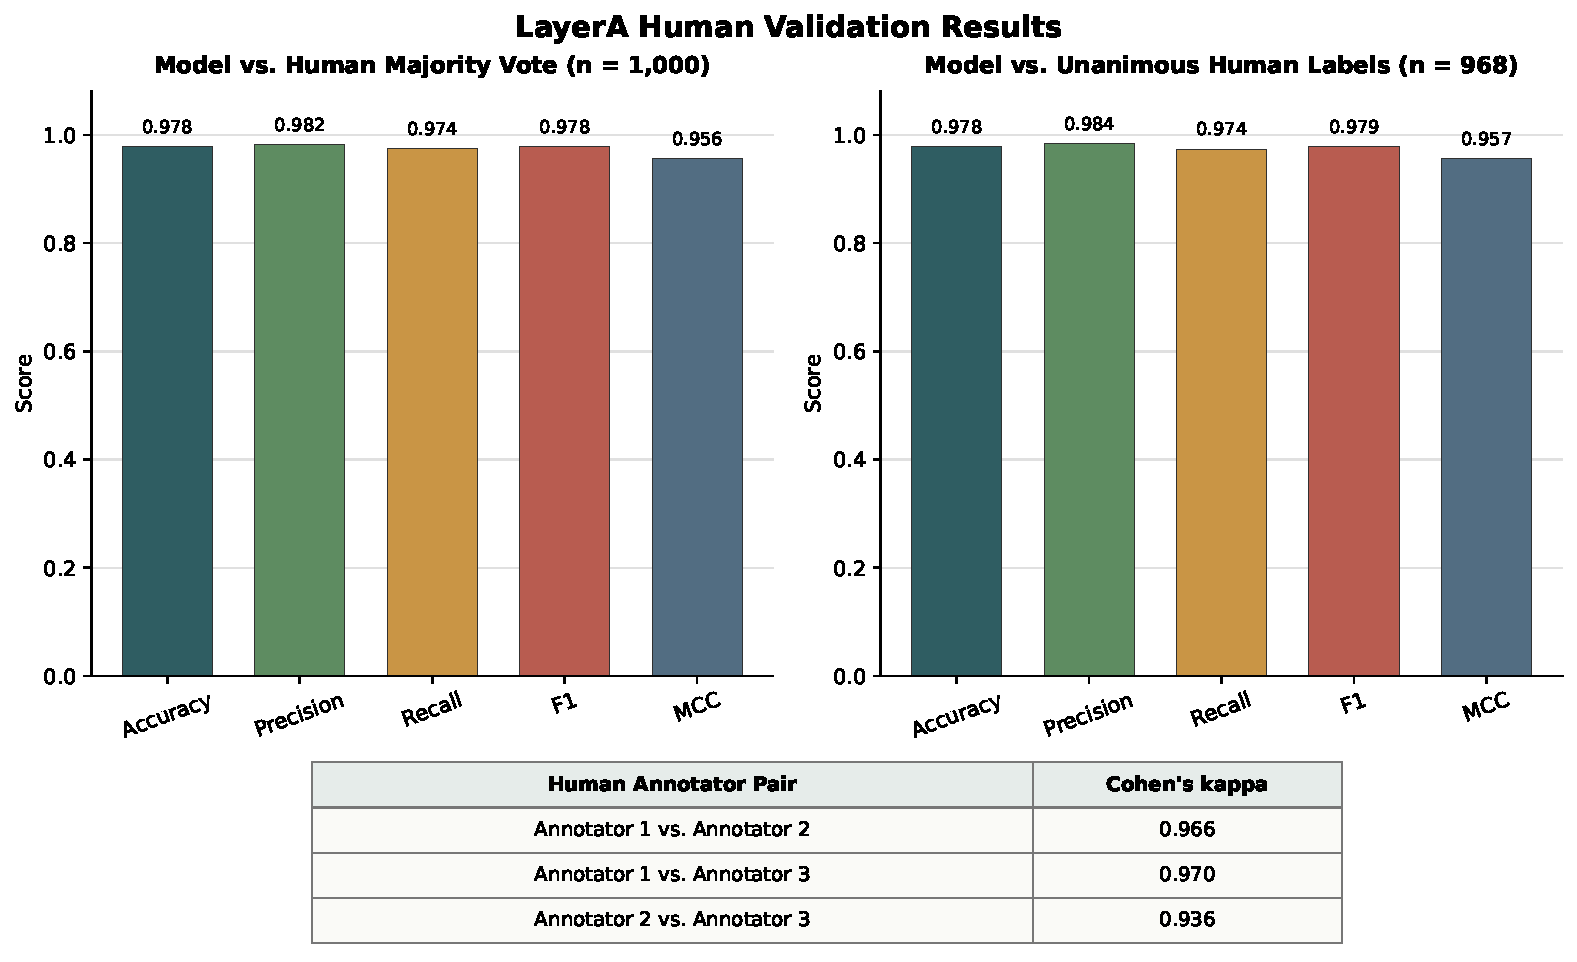
\includegraphics[width=0.85\textwidth]{figures/layer_a_validation.pdf}
    \caption{Layer A human-validation results. The bar charts compare model classifications with majority-vote and unanimous human labels; the table reports pairwise Cohen's kappa.}
    \label{fig:layer-a-validation-end}
\end{figure}

\begin{figure}[H]
    \centering
    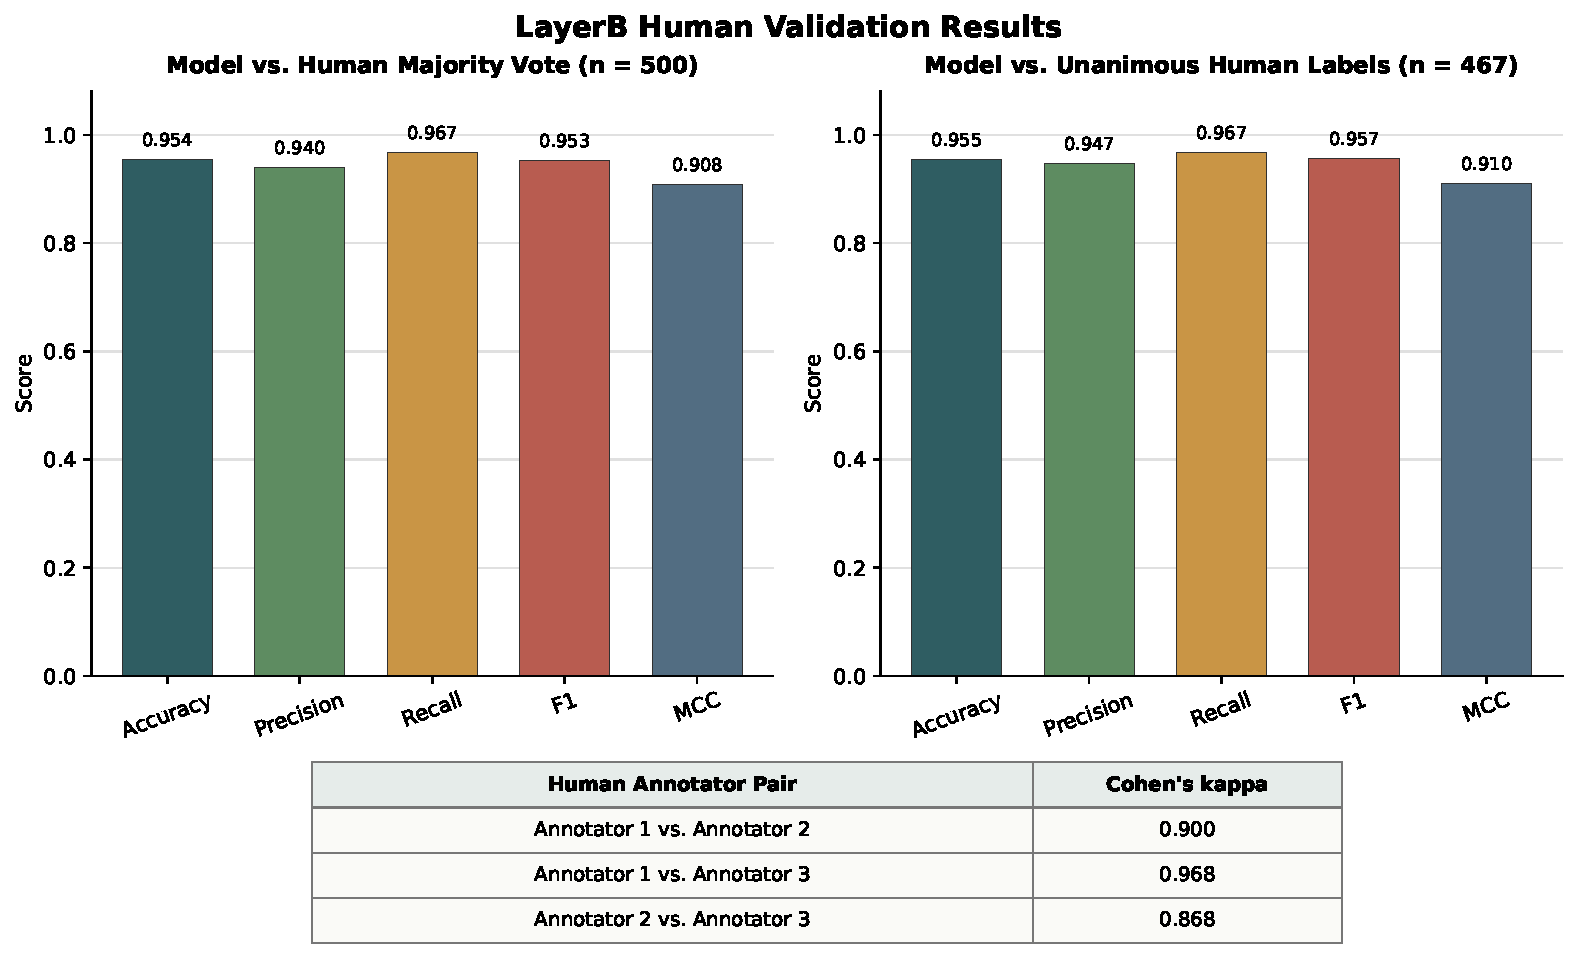
\includegraphics[width=0.85\textwidth]{figures/layer_b_validation.pdf}
    \caption{Layer B human-validation results. The bar charts compare model classifications with majority-vote and unanimous human labels; the table reports pairwise Cohen's kappa.}
    \label{fig:layer-b-validation-end}
\end{figure}

\section{Baseline Regression Robustness}
\label{sec:baseline-robustness}

The baseline regressions use firm-clustered standard errors. 
This appendix evaluates whether the inference is robust to alternative clustering choices. 
Industry--year two-way clustering allows dependence within industries and common shocks within years, while industry clustering provides a single-dimension benchmark that permits arbitrary within-industry dependence. 
The specifications retain the baseline sample, explanatory variables, controls, and year and industry fixed effects; only the standard-error estimator changes.

Table~\ref{tab:baseline_se_robustness} reports the results. The coefficient on \(IMS\) is \(-0.4829\) under all three clustering schemes. The standard errors and significance levels vary modestly, and \(IMS\) remains negative and statistically significant in each column. These results support the conclusion that the baseline association between audit-firm industry specialization and Greenwashing is not driven by the firm-clustered standard-error choice.

\begin{table}[H]
    \centering
    \caption{Robustness of Baseline Estimates to Alternative Standard-Error Clustering}
    \label{tab:baseline_se_robustness}
    \resizebox{0.9\textwidth}{!}{%
    \renewcommand{\arraystretch}{1.4}
    \begin{tabular}{lrrr}
        \toprule
        & (1) Firm-clustered SE & (2) Two-way clustered SE & (3) Industry-clustered SE \\
        \midrule
        \(IMS\) & \shortstack{-0.4829** \\ (0.2362)} & \shortstack{-0.4829** \\ (0.2348)} & \shortstack{-0.4829* \\ (0.2639)} \\
        Controls & Yes & Yes & Yes \\
        Observations & 15,381 & 15,381 & 15,381 \\
        Adjusted $R^2$ & 0.0221 & 0.0221 & 0.0221 \\
        Year fixed effects & Yes & Yes & Yes \\
        Industry fixed effects & Yes & Yes & Yes \\
        \bottomrule
    \end{tabular}%
    }
    \par\smallskip
    \begin{minipage}{0.95\textwidth}
        \footnotesize
        \textit{Notes:} The dependent variable is current Greenwashing. All columns estimate the baseline specification with the full set of financial, governance, and audit controls. Only the standard-error clustering changes across columns. Coefficient estimates are reported first, followed by standard errors in parentheses. ***, **, and * indicate two-tailed significance at 1, 5, and 10 percent.
    \end{minipage}
\end{table}


\section{Additional GPS Specifications}
\label{sec:gps-appendix}

Table~\ref{tab:gps-ipw-sensitivity} reports weight-trimming sensitivity for the same specification. 
The only difference across rows is the treatment of the estimated GPS weights. All GPS first-stage covariates are constructed after applying the baseline 1st--99th percentile winsorization to continuous controls in the complete baseline common sample.

The untrimmed specification retains every estimated weight and therefore preserves the original GPS reweighted target population, but it can be more sensitive to observations with relatively low conditional treatment density and unusually large weights. 
P0.5--P99.5 and P1--P99 trimming limits the influence of these extreme weights and increases the effective sample size, but it also changes the weighting scheme and hence the exact target pseudo-population. 
The negative coefficient remains similar across the three weight treatments, providing supplementary evidence that the main association is not driven solely by the most influential weights.

\begin{table}[H]
    \centering
    \caption{GPS--IPW Weight-Trimming Sensitivity}
    \label{tab:gps-ipw-sensitivity}
    \resizebox{0.9\textwidth}{!}{%
    \begin{tabular}{lrrrr}
        \toprule
        Weight treatment & \(IMS\) & Standard error & \(p\)-value & ESS \\
        \midrule
        Untrimmed & -0.2878 & 0.1191 & 0.0157 & 7,485 \\
        P0.5--P99.5 trimmed & -0.2351 & 0.1152 & 0.0413 & 8,529 \\
        P1--P99 trimmed & -0.2221 & 0.1147 & 0.0529 & 8,857 \\
        \bottomrule
    \end{tabular}%
    }
    \par\smallskip
    \begin{minipage}{0.95\textwidth}
        \footnotesize
        \textit{Notes:} All models use 10,488 firm-years and 4,168 firms, include year and industry fixed effects, and use firm-clustered standard errors. ESS is the effective sample size. Weight trimming is applied to the estimated GPS weights.
    \end{minipage}
\end{table}

Because \(IMS\) is continuous, the GPS--IPW analysis retains variation in specialization intensity. 
As a complementary check on observable selection, we recast specialization as the binary indicator \(IMS_D\) and re-estimate the association using entropy balancing \citep{hainmueller2012}
\footnote{We implement Hainmueller's (2012) ATT entropy balancing by reweighting untreated observations so that the first moments of the lagged financial, governance, and audit-selection covariates, and the second moments of the continuous lagged covariates, match the treated group.} and propensity-score matching \citep{minuttimeza2013,shipman2017psm}\footnote{Following Minutti-Meza (2013) and Shipman et al. (2017), we estimate a logit propensity-score model with the full set of lagged covariates, impose common support, and match treated and control observations 1:1 without replacement using a caliper of 0.03.}.
Table~\ref{tab:gps-binary-matching} reports the results. Column (1) uses entropy balancing and column (2) uses propensity-score matching. In both columns the coefficient remains negative and statistically significant, consistent with the GPS--IPW estimates.

\begin{table}[H]
    \centering
    \caption{Binary Complements to GPS--IPW}
    \label{tab:gps-binary-matching}
    \resizebox{0.9\textwidth}{!}{%
    \renewcommand{\arraystretch}{1.4}
    \begin{tabular}{lrr}
        \toprule
        & (1) Entropy Balancing & (2) Propensity-Score Matching \\
        \midrule
        \(IMS\) & \shortstack{-0.3406** \\ (0.1542)} & --- \\
        \(IMS_D\) & --- & \shortstack{-0.1120** \\ (0.0534)} \\
        Controls & Yes & Yes \\
        Observations & 10,488 & 1,218 \\
        Adjusted $R^2$ & 0.6079 & 0.5906 \\
        Year fixed effects & Yes & Yes \\
        Industry fixed effects & Yes & Yes \\
        \bottomrule
    \end{tabular}%
    }
    \par\smallskip
    \begin{minipage}{0.95\textwidth}
        \footnotesize
        \textit{Notes:} The dependent variable is current Greenwashing. Column (1) reports the entropy-balancing specification and column (2) reports the propensity-score matching specification. Coefficient estimates are reported first, followed by standard errors in parentheses. All models include year and industry fixed effects and use firm-clustered standard errors. Column (1) uses 10,488 firm-years from 4,168 firms; the effective sample size is 2,245. Column (2) uses 1,218 matched firm-years from 792 firms (609 pairs). ***, **, and * indicate two-tailed significance at 1, 5, and 10 percent.
    \end{minipage}
\end{table}


\end{document}
